\documentclass[twoside]{book}

% Packages required by doxygen
\usepackage{fixltx2e}
\usepackage{calc}
\usepackage{doxygen}
\usepackage[export]{adjustbox} % also loads graphicx
\usepackage{graphicx}
\usepackage[utf8]{inputenc}
\usepackage{makeidx}
\usepackage{multicol}
\usepackage{multirow}
\PassOptionsToPackage{warn}{textcomp}
\usepackage{textcomp}
\usepackage[nointegrals]{wasysym}
\usepackage[table]{xcolor}

% Font selection
\usepackage[T1]{fontenc}
\usepackage[scaled=.90]{helvet}
\usepackage{courier}
\usepackage{amssymb}
\usepackage{sectsty}
\renewcommand{\familydefault}{\sfdefault}
\allsectionsfont{%
  \fontseries{bc}\selectfont%
  \color{darkgray}%
}
\renewcommand{\DoxyLabelFont}{%
  \fontseries{bc}\selectfont%
  \color{darkgray}%
}
\newcommand{\+}{\discretionary{\mbox{\scriptsize$\hookleftarrow$}}{}{}}

% Page & text layout
\usepackage{geometry}
\geometry{%
  a4paper,%
  top=2.5cm,%
  bottom=2.5cm,%
  left=2.5cm,%
  right=2.5cm%
}
\tolerance=750
\hfuzz=15pt
\hbadness=750
\setlength{\emergencystretch}{15pt}
\setlength{\parindent}{0cm}
\setlength{\parskip}{3ex plus 2ex minus 2ex}
\makeatletter
\renewcommand{\paragraph}{%
  \@startsection{paragraph}{4}{0ex}{-1.0ex}{1.0ex}{%
    \normalfont\normalsize\bfseries\SS@parafont%
  }%
}
\renewcommand{\subparagraph}{%
  \@startsection{subparagraph}{5}{0ex}{-1.0ex}{1.0ex}{%
    \normalfont\normalsize\bfseries\SS@subparafont%
  }%
}
\makeatother

% Headers & footers
\usepackage{fancyhdr}
\pagestyle{fancyplain}
\fancyhead[LE]{\fancyplain{}{\bfseries\thepage}}
\fancyhead[CE]{\fancyplain{}{}}
\fancyhead[RE]{\fancyplain{}{\bfseries\leftmark}}
\fancyhead[LO]{\fancyplain{}{\bfseries\rightmark}}
\fancyhead[CO]{\fancyplain{}{}}
\fancyhead[RO]{\fancyplain{}{\bfseries\thepage}}
\fancyfoot[LE]{\fancyplain{}{}}
\fancyfoot[CE]{\fancyplain{}{}}
\fancyfoot[RE]{\fancyplain{}{\bfseries\scriptsize Generated by Doxygen }}
\fancyfoot[LO]{\fancyplain{}{\bfseries\scriptsize Generated by Doxygen }}
\fancyfoot[CO]{\fancyplain{}{}}
\fancyfoot[RO]{\fancyplain{}{}}
\renewcommand{\footrulewidth}{0.4pt}
\renewcommand{\chaptermark}[1]{%
  \markboth{#1}{}%
}
\renewcommand{\sectionmark}[1]{%
  \markright{\thesection\ #1}%
}

% Indices & bibliography
\usepackage{natbib}
\usepackage[titles]{tocloft}
\setcounter{tocdepth}{3}
\setcounter{secnumdepth}{5}
\makeindex

% Hyperlinks (required, but should be loaded last)
\usepackage{ifpdf}
\ifpdf
  \usepackage[pdftex,pagebackref=true]{hyperref}
\else
  \usepackage[ps2pdf,pagebackref=true]{hyperref}
\fi
\hypersetup{%
  colorlinks=true,%
  linkcolor=blue,%
  citecolor=blue,%
  unicode%
}

% Custom commands
\newcommand{\clearemptydoublepage}{%
  \newpage{\pagestyle{empty}\cleardoublepage}%
}

\usepackage{caption}
\captionsetup{labelsep=space,justification=centering,font={bf},singlelinecheck=off,skip=4pt,position=top}

%===== C O N T E N T S =====

\begin{document}

% Titlepage & ToC
\hypersetup{pageanchor=false,
             bookmarksnumbered=true,
             pdfencoding=unicode
            }
\pagenumbering{alph}
\begin{titlepage}
\vspace*{7cm}
\begin{center}%
{\Large Application de planification de vols aériens }\\
\vspace*{1cm}
{\large Generated by Doxygen 1.8.13}\\
\end{center}
\end{titlepage}
\clearemptydoublepage
\pagenumbering{roman}
\tableofcontents
\clearemptydoublepage
\pagenumbering{arabic}
\hypersetup{pageanchor=true}

%--- Begin generated contents ---
\chapter{Namespace Index}
\section{Packages}
Here are the packages with brief descriptions (if available)\+:\begin{DoxyCompactList}
\item\contentsline{section}{\hyperlink{namespace_application__de__planification__de__vols__a_xC3_xA9riens}{Application\+\_\+de\+\_\+planification\+\_\+de\+\_\+vols\+\_\+aériens} }{\pageref{namespace_application__de__planification__de__vols__a_xC3_xA9riens}}{}
\end{DoxyCompactList}

\chapter{Hierarchical Index}
\section{Class Hierarchy}
This inheritance list is sorted roughly, but not completely, alphabetically\+:\begin{DoxyCompactList}
\item \contentsline{section}{Application\+\_\+de\+\_\+planification\+\_\+de\+\_\+vols\+\_\+aériens.\+Airport}{\pageref{class_application__de__planification__de__vols__a_xC3_xA9riens_1_1_airport}}{}
\item \contentsline{section}{Application\+\_\+de\+\_\+planification\+\_\+de\+\_\+vols\+\_\+aériens.\+D\+B\+Connexion}{\pageref{class_application__de__planification__de__vols__a_xC3_xA9riens_1_1_d_b_connexion}}{}
\item \contentsline{section}{Application\+\_\+de\+\_\+planification\+\_\+de\+\_\+vols\+\_\+aériens.\+Flight}{\pageref{class_application__de__planification__de__vols__a_xC3_xA9riens_1_1_flight}}{}
\item \contentsline{section}{Application\+\_\+de\+\_\+planification\+\_\+de\+\_\+vols\+\_\+aériens.\+Flight\+Schedule}{\pageref{class_application__de__planification__de__vols__a_xC3_xA9riens_1_1_flight_schedule}}{}
\item Form\begin{DoxyCompactList}
\item \contentsline{section}{Application\+\_\+de\+\_\+planification\+\_\+de\+\_\+vols\+\_\+aériens.\+Affichage}{\pageref{class_application__de__planification__de__vols__a_xC3_xA9riens_1_1_affichage}}{}
\item \contentsline{section}{Application\+\_\+de\+\_\+planification\+\_\+de\+\_\+vols\+\_\+aériens.\+frm\+Affectation\+Vol}{\pageref{class_application__de__planification__de__vols__a_xC3_xA9riens_1_1frm_affectation_vol}}{}
\item \contentsline{section}{Application\+\_\+de\+\_\+planification\+\_\+de\+\_\+vols\+\_\+aériens.\+frm\+Gestion}{\pageref{class_application__de__planification__de__vols__a_xC3_xA9riens_1_1frm_gestion}}{}
\item \contentsline{section}{Application\+\_\+de\+\_\+planification\+\_\+de\+\_\+vols\+\_\+aériens.\+frm\+Vacances}{\pageref{class_application__de__planification__de__vols__a_xC3_xA9riens_1_1frm_vacances}}{}
\item \contentsline{section}{Application\+\_\+de\+\_\+planification\+\_\+de\+\_\+vols\+\_\+aériens.\+frm\+Vacances\+Affichage}{\pageref{class_application__de__planification__de__vols__a_xC3_xA9riens_1_1frm_vacances_affichage}}{}
\end{DoxyCompactList}
\item \contentsline{section}{Application\+\_\+de\+\_\+planification\+\_\+de\+\_\+vols\+\_\+aériens.\+Line}{\pageref{class_application__de__planification__de__vols__a_xC3_xA9riens_1_1_line}}{}
\item \contentsline{section}{Application\+\_\+de\+\_\+planification\+\_\+de\+\_\+vols\+\_\+aériens.\+Pilot}{\pageref{class_application__de__planification__de__vols__a_xC3_xA9riens_1_1_pilot}}{}
\item \contentsline{section}{Application\+\_\+de\+\_\+planification\+\_\+de\+\_\+vols\+\_\+aériens.\+Program}{\pageref{class_application__de__planification__de__vols__a_xC3_xA9riens_1_1_program}}{}
\item \contentsline{section}{Application\+\_\+de\+\_\+planification\+\_\+de\+\_\+vols\+\_\+aériens.\+Vacation}{\pageref{class_application__de__planification__de__vols__a_xC3_xA9riens_1_1_vacation}}{}
\end{DoxyCompactList}

\chapter{Class Index}
\section{Class List}
Here are the classes, structs, unions and interfaces with brief descriptions\+:\begin{DoxyCompactList}
\item\contentsline{section}{\hyperlink{class_application__de__planification__de__vols__a_xC3_xA9riens_1_1_affichage}{Application\+\_\+de\+\_\+planification\+\_\+de\+\_\+vols\+\_\+aériens.\+Affichage} }{\pageref{class_application__de__planification__de__vols__a_xC3_xA9riens_1_1_affichage}}{}
\item\contentsline{section}{\hyperlink{class_application__de__planification__de__vols__a_xC3_xA9riens_1_1_airport}{Application\+\_\+de\+\_\+planification\+\_\+de\+\_\+vols\+\_\+aériens.\+Airport} }{\pageref{class_application__de__planification__de__vols__a_xC3_xA9riens_1_1_airport}}{}
\item\contentsline{section}{\hyperlink{class_application__de__planification__de__vols__a_xC3_xA9riens_1_1_d_b_connexion}{Application\+\_\+de\+\_\+planification\+\_\+de\+\_\+vols\+\_\+aériens.\+D\+B\+Connexion} }{\pageref{class_application__de__planification__de__vols__a_xC3_xA9riens_1_1_d_b_connexion}}{}
\item\contentsline{section}{\hyperlink{class_application__de__planification__de__vols__a_xC3_xA9riens_1_1_flight}{Application\+\_\+de\+\_\+planification\+\_\+de\+\_\+vols\+\_\+aériens.\+Flight} }{\pageref{class_application__de__planification__de__vols__a_xC3_xA9riens_1_1_flight}}{}
\item\contentsline{section}{\hyperlink{class_application__de__planification__de__vols__a_xC3_xA9riens_1_1_flight_schedule}{Application\+\_\+de\+\_\+planification\+\_\+de\+\_\+vols\+\_\+aériens.\+Flight\+Schedule} }{\pageref{class_application__de__planification__de__vols__a_xC3_xA9riens_1_1_flight_schedule}}{}
\item\contentsline{section}{\hyperlink{class_application__de__planification__de__vols__a_xC3_xA9riens_1_1frm_affectation_vol}{Application\+\_\+de\+\_\+planification\+\_\+de\+\_\+vols\+\_\+aériens.\+frm\+Affectation\+Vol} }{\pageref{class_application__de__planification__de__vols__a_xC3_xA9riens_1_1frm_affectation_vol}}{}
\item\contentsline{section}{\hyperlink{class_application__de__planification__de__vols__a_xC3_xA9riens_1_1frm_gestion}{Application\+\_\+de\+\_\+planification\+\_\+de\+\_\+vols\+\_\+aériens.\+frm\+Gestion} }{\pageref{class_application__de__planification__de__vols__a_xC3_xA9riens_1_1frm_gestion}}{}
\item\contentsline{section}{\hyperlink{class_application__de__planification__de__vols__a_xC3_xA9riens_1_1frm_vacances}{Application\+\_\+de\+\_\+planification\+\_\+de\+\_\+vols\+\_\+aériens.\+frm\+Vacances} }{\pageref{class_application__de__planification__de__vols__a_xC3_xA9riens_1_1frm_vacances}}{}
\item\contentsline{section}{\hyperlink{class_application__de__planification__de__vols__a_xC3_xA9riens_1_1frm_vacances_affichage}{Application\+\_\+de\+\_\+planification\+\_\+de\+\_\+vols\+\_\+aériens.\+frm\+Vacances\+Affichage} }{\pageref{class_application__de__planification__de__vols__a_xC3_xA9riens_1_1frm_vacances_affichage}}{}
\item\contentsline{section}{\hyperlink{class_application__de__planification__de__vols__a_xC3_xA9riens_1_1_line}{Application\+\_\+de\+\_\+planification\+\_\+de\+\_\+vols\+\_\+aériens.\+Line} }{\pageref{class_application__de__planification__de__vols__a_xC3_xA9riens_1_1_line}}{}
\item\contentsline{section}{\hyperlink{class_application__de__planification__de__vols__a_xC3_xA9riens_1_1_pilot}{Application\+\_\+de\+\_\+planification\+\_\+de\+\_\+vols\+\_\+aériens.\+Pilot} }{\pageref{class_application__de__planification__de__vols__a_xC3_xA9riens_1_1_pilot}}{}
\item\contentsline{section}{\hyperlink{class_application__de__planification__de__vols__a_xC3_xA9riens_1_1_program}{Application\+\_\+de\+\_\+planification\+\_\+de\+\_\+vols\+\_\+aériens.\+Program} }{\pageref{class_application__de__planification__de__vols__a_xC3_xA9riens_1_1_program}}{}
\item\contentsline{section}{\hyperlink{class_application__de__planification__de__vols__a_xC3_xA9riens_1_1_vacation}{Application\+\_\+de\+\_\+planification\+\_\+de\+\_\+vols\+\_\+aériens.\+Vacation} }{\pageref{class_application__de__planification__de__vols__a_xC3_xA9riens_1_1_vacation}}{}
\end{DoxyCompactList}

\chapter{File Index}
\section{File List}
Here is a list of all files with brief descriptions\+:\begin{DoxyCompactList}
\item\contentsline{section}{Application de planification de vols aériens/\hyperlink{_airport_8cs}{Airport.\+cs} }{\pageref{_airport_8cs}}{}
\item\contentsline{section}{Application de planification de vols aériens/\hyperlink{_d_b_connexion_8cs}{D\+B\+Connexion.\+cs} }{\pageref{_d_b_connexion_8cs}}{}
\item\contentsline{section}{Application de planification de vols aériens/\hyperlink{_flight_8cs}{Flight.\+cs} }{\pageref{_flight_8cs}}{}
\item\contentsline{section}{Application de planification de vols aériens/\hyperlink{_flight_schedule_8cs}{Flight\+Schedule.\+cs} }{\pageref{_flight_schedule_8cs}}{}
\item\contentsline{section}{Application de planification de vols aériens/\hyperlink{frm_affectation_vol_8cs}{frm\+Affectation\+Vol.\+cs} }{\pageref{frm_affectation_vol_8cs}}{}
\item\contentsline{section}{Application de planification de vols aériens/\hyperlink{frm_affectation_vol_8_designer_8cs}{frm\+Affectation\+Vol.\+Designer.\+cs} }{\pageref{frm_affectation_vol_8_designer_8cs}}{}
\item\contentsline{section}{Application de planification de vols aériens/\hyperlink{frm_affichage_8cs}{frm\+Affichage.\+cs} }{\pageref{frm_affichage_8cs}}{}
\item\contentsline{section}{Application de planification de vols aériens/\hyperlink{frm_affichage_8_designer_8cs}{frm\+Affichage.\+Designer.\+cs} }{\pageref{frm_affichage_8_designer_8cs}}{}
\item\contentsline{section}{Application de planification de vols aériens/\hyperlink{frm_gestion_8cs}{frm\+Gestion.\+cs} }{\pageref{frm_gestion_8cs}}{}
\item\contentsline{section}{Application de planification de vols aériens/\hyperlink{frm_gestion_8_designer_8cs}{frm\+Gestion.\+Designer.\+cs} }{\pageref{frm_gestion_8_designer_8cs}}{}
\item\contentsline{section}{Application de planification de vols aériens/\hyperlink{frm_vacances_8cs}{frm\+Vacances.\+cs} }{\pageref{frm_vacances_8cs}}{}
\item\contentsline{section}{Application de planification de vols aériens/\hyperlink{frm_vacances_8_designer_8cs}{frm\+Vacances.\+Designer.\+cs} }{\pageref{frm_vacances_8_designer_8cs}}{}
\item\contentsline{section}{Application de planification de vols aériens/\hyperlink{frm_vacances_affichage_8cs}{frm\+Vacances\+Affichage.\+cs} }{\pageref{frm_vacances_affichage_8cs}}{}
\item\contentsline{section}{Application de planification de vols aériens/\hyperlink{frm_vacances_affichage_8_designer_8cs}{frm\+Vacances\+Affichage.\+Designer.\+cs} }{\pageref{frm_vacances_affichage_8_designer_8cs}}{}
\item\contentsline{section}{Application de planification de vols aériens/\hyperlink{_line_8cs}{Line.\+cs} }{\pageref{_line_8cs}}{}
\item\contentsline{section}{Application de planification de vols aériens/\hyperlink{_pilot_8cs}{Pilot.\+cs} }{\pageref{_pilot_8cs}}{}
\item\contentsline{section}{Application de planification de vols aériens/\hyperlink{_program_8cs}{Program.\+cs} }{\pageref{_program_8cs}}{}
\item\contentsline{section}{Application de planification de vols aériens/\hyperlink{_vacation_8cs}{Vacation.\+cs} }{\pageref{_vacation_8cs}}{}
\end{DoxyCompactList}

\chapter{Namespace Documentation}
\hypertarget{namespace_application__de__planification__de__vols__a_xC3_xA9riens}{}\section{Application\+\_\+de\+\_\+planification\+\_\+de\+\_\+vols\+\_\+aériens Namespace Reference}
\label{namespace_application__de__planification__de__vols__a_xC3_xA9riens}\index{Application\+\_\+de\+\_\+planification\+\_\+de\+\_\+vols\+\_\+aériens@{Application\+\_\+de\+\_\+planification\+\_\+de\+\_\+vols\+\_\+aériens}}
\subsection*{Classes}
\begin{DoxyCompactItemize}
\item 
class \hyperlink{class_application__de__planification__de__vols__a_xC3_xA9riens_1_1_affichage}{Affichage}
\item 
class \hyperlink{class_application__de__planification__de__vols__a_xC3_xA9riens_1_1_airport}{Airport}
\item 
class \hyperlink{class_application__de__planification__de__vols__a_xC3_xA9riens_1_1_d_b_connexion}{D\+B\+Connexion}
\item 
class \hyperlink{class_application__de__planification__de__vols__a_xC3_xA9riens_1_1_flight}{Flight}
\item 
class \hyperlink{class_application__de__planification__de__vols__a_xC3_xA9riens_1_1_flight_schedule}{Flight\+Schedule}
\item 
class \hyperlink{class_application__de__planification__de__vols__a_xC3_xA9riens_1_1frm_affectation_vol}{frm\+Affectation\+Vol}
\item 
class \hyperlink{class_application__de__planification__de__vols__a_xC3_xA9riens_1_1frm_gestion}{frm\+Gestion}
\item 
class \hyperlink{class_application__de__planification__de__vols__a_xC3_xA9riens_1_1frm_vacances}{frm\+Vacances}
\item 
class \hyperlink{class_application__de__planification__de__vols__a_xC3_xA9riens_1_1frm_vacances_affichage}{frm\+Vacances\+Affichage}
\item 
class \hyperlink{class_application__de__planification__de__vols__a_xC3_xA9riens_1_1_line}{Line}
\item 
class \hyperlink{class_application__de__planification__de__vols__a_xC3_xA9riens_1_1_pilot}{Pilot}
\item 
class \hyperlink{class_application__de__planification__de__vols__a_xC3_xA9riens_1_1_program}{Program}
\item 
class \hyperlink{class_application__de__planification__de__vols__a_xC3_xA9riens_1_1_vacation}{Vacation}
\end{DoxyCompactItemize}

\chapter{Class Documentation}
\hypertarget{class_application__de__planification__de__vols__a_xC3_xA9riens_1_1_affichage}{}\section{Application\+\_\+de\+\_\+planification\+\_\+de\+\_\+vols\+\_\+aériens.\+Affichage Class Reference}
\label{class_application__de__planification__de__vols__a_xC3_xA9riens_1_1_affichage}\index{Application\+\_\+de\+\_\+planification\+\_\+de\+\_\+vols\+\_\+aériens.\+Affichage@{Application\+\_\+de\+\_\+planification\+\_\+de\+\_\+vols\+\_\+aériens.\+Affichage}}
Inheritance diagram for Application\+\_\+de\+\_\+planification\+\_\+de\+\_\+vols\+\_\+aériens.\+Affichage\+:\begin{figure}[H]
\begin{center}
\leavevmode
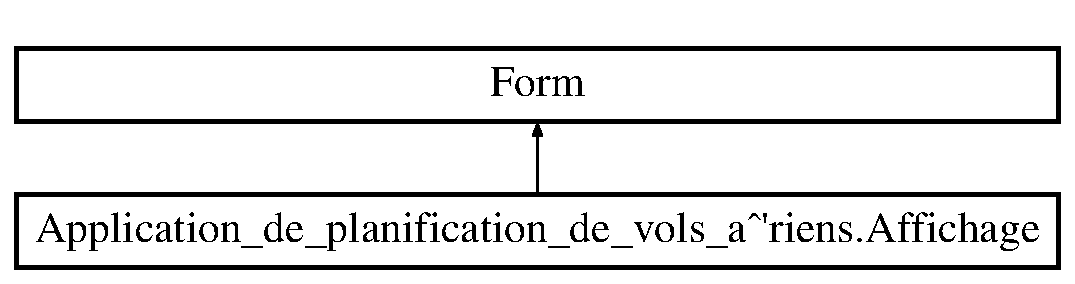
\includegraphics[height=2.000000cm]{class_application__de__planification__de__vols__a_xC3_xA9riens_1_1_affichage}
\end{center}
\end{figure}
\subsection*{Public Member Functions}
\begin{DoxyCompactItemize}
\item 
\hyperlink{class_application__de__planification__de__vols__a_xC3_xA9riens_1_1_affichage_a224f6dc223876b40e7ae776207a269b7}{Affichage} ()
\end{DoxyCompactItemize}
\subsection*{Protected Member Functions}
\begin{DoxyCompactItemize}
\item 
override void \hyperlink{class_application__de__planification__de__vols__a_xC3_xA9riens_1_1_affichage_addb34a9fdcc33294a51e6b0012ab89a7}{Dispose} (bool disposing)
\begin{DoxyCompactList}\small\item\em Clean up any resources being used. \end{DoxyCompactList}\end{DoxyCompactItemize}


\subsection{Constructor \& Destructor Documentation}
\mbox{\Hypertarget{class_application__de__planification__de__vols__a_xC3_xA9riens_1_1_affichage_a224f6dc223876b40e7ae776207a269b7}\label{class_application__de__planification__de__vols__a_xC3_xA9riens_1_1_affichage_a224f6dc223876b40e7ae776207a269b7}} 
\index{Application\+\_\+de\+\_\+planification\+\_\+de\+\_\+vols\+\_\+aériens\+::\+Affichage@{Application\+\_\+de\+\_\+planification\+\_\+de\+\_\+vols\+\_\+aériens\+::\+Affichage}!Affichage@{Affichage}}
\index{Affichage@{Affichage}!Application\+\_\+de\+\_\+planification\+\_\+de\+\_\+vols\+\_\+aériens\+::\+Affichage@{Application\+\_\+de\+\_\+planification\+\_\+de\+\_\+vols\+\_\+aériens\+::\+Affichage}}
\subsubsection{\texorpdfstring{Affichage()}{Affichage()}}
{\footnotesize\ttfamily Application\+\_\+de\+\_\+planification\+\_\+de\+\_\+vols\+\_\+aériens.\+Affichage.\+Affichage (\begin{DoxyParamCaption}{ }\end{DoxyParamCaption})}



\subsection{Member Function Documentation}
\mbox{\Hypertarget{class_application__de__planification__de__vols__a_xC3_xA9riens_1_1_affichage_addb34a9fdcc33294a51e6b0012ab89a7}\label{class_application__de__planification__de__vols__a_xC3_xA9riens_1_1_affichage_addb34a9fdcc33294a51e6b0012ab89a7}} 
\index{Application\+\_\+de\+\_\+planification\+\_\+de\+\_\+vols\+\_\+aériens\+::\+Affichage@{Application\+\_\+de\+\_\+planification\+\_\+de\+\_\+vols\+\_\+aériens\+::\+Affichage}!Dispose@{Dispose}}
\index{Dispose@{Dispose}!Application\+\_\+de\+\_\+planification\+\_\+de\+\_\+vols\+\_\+aériens\+::\+Affichage@{Application\+\_\+de\+\_\+planification\+\_\+de\+\_\+vols\+\_\+aériens\+::\+Affichage}}
\subsubsection{\texorpdfstring{Dispose()}{Dispose()}}
{\footnotesize\ttfamily override void Application\+\_\+de\+\_\+planification\+\_\+de\+\_\+vols\+\_\+aériens.\+Affichage.\+Dispose (\begin{DoxyParamCaption}\item[{bool}]{disposing }\end{DoxyParamCaption})\hspace{0.3cm}{\ttfamily [protected]}}



Clean up any resources being used. 


\begin{DoxyParams}{Parameters}
{\em disposing} & true if managed resources should be disposed; otherwise, false.\\
\hline
\end{DoxyParams}


The documentation for this class was generated from the following files\+:\begin{DoxyCompactItemize}
\item 
Application de planification de vols aériens/\hyperlink{frm_affichage_8cs}{frm\+Affichage.\+cs}\item 
Application de planification de vols aériens/\hyperlink{frm_affichage_8_designer_8cs}{frm\+Affichage.\+Designer.\+cs}\end{DoxyCompactItemize}

\hypertarget{class_application__de__planification__de__vols__a_xC3_xA9riens_1_1_airport}{}\section{Application\+\_\+de\+\_\+planification\+\_\+de\+\_\+vols\+\_\+aériens.\+Airport Class Reference}
\label{class_application__de__planification__de__vols__a_xC3_xA9riens_1_1_airport}\index{Application\+\_\+de\+\_\+planification\+\_\+de\+\_\+vols\+\_\+aériens.\+Airport@{Application\+\_\+de\+\_\+planification\+\_\+de\+\_\+vols\+\_\+aériens.\+Airport}}
\subsection*{Public Member Functions}
\begin{DoxyCompactItemize}
\item 
\hyperlink{class_application__de__planification__de__vols__a_xC3_xA9riens_1_1_airport_a5507521a7e89a1cef679eff2a043f89c}{Airport} (string name)
\end{DoxyCompactItemize}
\subsection*{Properties}
\begin{DoxyCompactItemize}
\item 
string \hyperlink{class_application__de__planification__de__vols__a_xC3_xA9riens_1_1_airport_a25b8937bd4f555b7597bd2ac771da73d}{Name}\hspace{0.3cm}{\ttfamily  \mbox{[}get, set\mbox{]}}
\end{DoxyCompactItemize}


\subsection{Constructor \& Destructor Documentation}
\mbox{\Hypertarget{class_application__de__planification__de__vols__a_xC3_xA9riens_1_1_airport_a5507521a7e89a1cef679eff2a043f89c}\label{class_application__de__planification__de__vols__a_xC3_xA9riens_1_1_airport_a5507521a7e89a1cef679eff2a043f89c}} 
\index{Application\+\_\+de\+\_\+planification\+\_\+de\+\_\+vols\+\_\+aériens\+::\+Airport@{Application\+\_\+de\+\_\+planification\+\_\+de\+\_\+vols\+\_\+aériens\+::\+Airport}!Airport@{Airport}}
\index{Airport@{Airport}!Application\+\_\+de\+\_\+planification\+\_\+de\+\_\+vols\+\_\+aériens\+::\+Airport@{Application\+\_\+de\+\_\+planification\+\_\+de\+\_\+vols\+\_\+aériens\+::\+Airport}}
\subsubsection{\texorpdfstring{Airport()}{Airport()}}
{\footnotesize\ttfamily Application\+\_\+de\+\_\+planification\+\_\+de\+\_\+vols\+\_\+aériens.\+Airport.\+Airport (\begin{DoxyParamCaption}\item[{string}]{name }\end{DoxyParamCaption})}



\subsection{Property Documentation}
\mbox{\Hypertarget{class_application__de__planification__de__vols__a_xC3_xA9riens_1_1_airport_a25b8937bd4f555b7597bd2ac771da73d}\label{class_application__de__planification__de__vols__a_xC3_xA9riens_1_1_airport_a25b8937bd4f555b7597bd2ac771da73d}} 
\index{Application\+\_\+de\+\_\+planification\+\_\+de\+\_\+vols\+\_\+aériens\+::\+Airport@{Application\+\_\+de\+\_\+planification\+\_\+de\+\_\+vols\+\_\+aériens\+::\+Airport}!Name@{Name}}
\index{Name@{Name}!Application\+\_\+de\+\_\+planification\+\_\+de\+\_\+vols\+\_\+aériens\+::\+Airport@{Application\+\_\+de\+\_\+planification\+\_\+de\+\_\+vols\+\_\+aériens\+::\+Airport}}
\subsubsection{\texorpdfstring{Name}{Name}}
{\footnotesize\ttfamily string Application\+\_\+de\+\_\+planification\+\_\+de\+\_\+vols\+\_\+aériens.\+Airport.\+Name\hspace{0.3cm}{\ttfamily [get]}, {\ttfamily [set]}}



The documentation for this class was generated from the following file\+:\begin{DoxyCompactItemize}
\item 
Application de planification de vols aériens/\hyperlink{_airport_8cs}{Airport.\+cs}\end{DoxyCompactItemize}

\hypertarget{class_application__de__planification__de__vols__a_xC3_xA9riens_1_1_d_b_connexion}{}\section{Application\+\_\+de\+\_\+planification\+\_\+de\+\_\+vols\+\_\+aériens.\+D\+B\+Connexion Class Reference}
\label{class_application__de__planification__de__vols__a_xC3_xA9riens_1_1_d_b_connexion}\index{Application\+\_\+de\+\_\+planification\+\_\+de\+\_\+vols\+\_\+aériens.\+D\+B\+Connexion@{Application\+\_\+de\+\_\+planification\+\_\+de\+\_\+vols\+\_\+aériens.\+D\+B\+Connexion}}
\subsection*{Public Member Functions}
\begin{DoxyCompactItemize}
\item 
\hyperlink{class_application__de__planification__de__vols__a_xC3_xA9riens_1_1_d_b_connexion_a9b5698ceb5adf9b44a745d830bf2ecaf}{D\+B\+Connexion} ()
\item 
void \hyperlink{class_application__de__planification__de__vols__a_xC3_xA9riens_1_1_d_b_connexion_aa9caece339aea7484598a37e50ca8af6}{Add\+Pilot} (\hyperlink{class_application__de__planification__de__vols__a_xC3_xA9riens_1_1_pilot}{Pilot} pilot)
\begin{DoxyCompactList}\small\item\em Add a pilot in db \end{DoxyCompactList}\item 
void \hyperlink{class_application__de__planification__de__vols__a_xC3_xA9riens_1_1_d_b_connexion_a2f4fd2e7c23839b549420fcca353984d}{Add\+Flight} (\hyperlink{class_application__de__planification__de__vols__a_xC3_xA9riens_1_1_flight}{Flight} flight)
\begin{DoxyCompactList}\small\item\em Add a flight in db \end{DoxyCompactList}\item 
void \hyperlink{class_application__de__planification__de__vols__a_xC3_xA9riens_1_1_d_b_connexion_a71d2d525cf37d0dc43f22efd89b82734}{Add\+Line} (\hyperlink{class_application__de__planification__de__vols__a_xC3_xA9riens_1_1_line}{Line} line)
\begin{DoxyCompactList}\small\item\em add a line in db \end{DoxyCompactList}\item 
void \hyperlink{class_application__de__planification__de__vols__a_xC3_xA9riens_1_1_d_b_connexion_a220f45595bbd59eaaabbbd898f7c73b1}{Add\+Vacation} (\hyperlink{class_application__de__planification__de__vols__a_xC3_xA9riens_1_1_vacation}{Vacation} vacation)
\begin{DoxyCompactList}\small\item\em add a vacation in db \end{DoxyCompactList}\item 
string \hyperlink{class_application__de__planification__de__vols__a_xC3_xA9riens_1_1_d_b_connexion_aba4d1644a2d30d5ecec7bf4dfa3a9331}{Get\+Airport\+Name} ()
\begin{DoxyCompactList}\small\item\em Retourne les noms des aéroports \end{DoxyCompactList}\item 
string \hyperlink{class_application__de__planification__de__vols__a_xC3_xA9riens_1_1_d_b_connexion_ad9fb77da79aa2d8b9f355e0638e0770a}{Get\+Line\+Name} ()
\begin{DoxyCompactList}\small\item\em Retourne le nom d\textquotesingle{}une ligne \end{DoxyCompactList}\item 
List$<$ \hyperlink{class_application__de__planification__de__vols__a_xC3_xA9riens_1_1_pilot}{Pilot} $>$ \hyperlink{class_application__de__planification__de__vols__a_xC3_xA9riens_1_1_d_b_connexion_a088f14b6281bd4ec62ffca81b04b2b84}{Get\+Pilots} ()
\item 
string \hyperlink{class_application__de__planification__de__vols__a_xC3_xA9riens_1_1_d_b_connexion_a54fe211e972cce80cc572dd73322dba3}{Get\+Pilot\+Name} ()
\item 
string \hyperlink{class_application__de__planification__de__vols__a_xC3_xA9riens_1_1_d_b_connexion_a45bd44b25fcaa50b31b0353e3fbe2666}{Get\+Pilot\+First\+Name} ()
\item 
string \hyperlink{class_application__de__planification__de__vols__a_xC3_xA9riens_1_1_d_b_connexion_ad4c54e9be3d1531491787d5ded6b98f0}{Get\+Pilot\+Assignment\+Airport} ()
\item 
int \hyperlink{class_application__de__planification__de__vols__a_xC3_xA9riens_1_1_d_b_connexion_a718b3ee189f7a5ff6f619f7061bd745d}{Get\+Pilot\+Flight\+Time} ()
\item 
string \hyperlink{class_application__de__planification__de__vols__a_xC3_xA9riens_1_1_d_b_connexion_a70816da17c8de039c2494e09102d9c00}{Get\+Pilot\+Current\+Location} ()
\item 
Date\+Time \hyperlink{class_application__de__planification__de__vols__a_xC3_xA9riens_1_1_d_b_connexion_a8b0816e5f3658817d4c1179b8c539483}{Get\+Pilot\+Last\+Flight\+Date} ()
\item 
Date\+Time \hyperlink{class_application__de__planification__de__vols__a_xC3_xA9riens_1_1_d_b_connexion_ac7dfc1290ea2ce940be274fd0184fc94}{Get\+Pilot\+Flights\+Departure\+Dates} ()
\item 
Date\+Time \hyperlink{class_application__de__planification__de__vols__a_xC3_xA9riens_1_1_d_b_connexion_aa30d1b13562f9f98aa57c9466e359d9b}{Get\+Pilot\+Flights\+Arrival\+Dates} ()
\item 
int \hyperlink{class_application__de__planification__de__vols__a_xC3_xA9riens_1_1_d_b_connexion_aa600049403e7f58b2a8c83586e7bde6d}{Get\+Pilot\+Id} (string pilot\+Name)
\item 
List$<$ \hyperlink{class_application__de__planification__de__vols__a_xC3_xA9riens_1_1_flight}{Flight} $>$ \hyperlink{class_application__de__planification__de__vols__a_xC3_xA9riens_1_1_d_b_connexion_a03271776c690de0248c0fbe84bf66c36}{Get\+Flights} ()
\item 
string \hyperlink{class_application__de__planification__de__vols__a_xC3_xA9riens_1_1_d_b_connexion_a4ca6ed28fb9d0169b5504acf754c2dd7}{Get\+Flight\+Name} ()
\item 
string \hyperlink{class_application__de__planification__de__vols__a_xC3_xA9riens_1_1_d_b_connexion_aacd19b3599d60ce5e027b74b1dc54ca2}{Get\+Flight\+Line} ()
\item 
Date\+Time \hyperlink{class_application__de__planification__de__vols__a_xC3_xA9riens_1_1_d_b_connexion_a2d5edf54c674ce7006e8ce528d2be882}{Get\+Departure\+Date} ()
\item 
Date\+Time \hyperlink{class_application__de__planification__de__vols__a_xC3_xA9riens_1_1_d_b_connexion_a3bdd8b23069a72ee3d040f9a4ea51992}{Get\+Arrival\+Date} ()
\item 
string \hyperlink{class_application__de__planification__de__vols__a_xC3_xA9riens_1_1_d_b_connexion_ae66e1cddbb79a1ce7228f634cd4bf284}{Get\+Flight\+Pilots} ()
\item 
List$<$ \hyperlink{class_application__de__planification__de__vols__a_xC3_xA9riens_1_1_line}{Line} $>$ \hyperlink{class_application__de__planification__de__vols__a_xC3_xA9riens_1_1_d_b_connexion_a87d99db67f6f29a892e4976394873bee}{Get\+Lines} ()
\item 
string \hyperlink{class_application__de__planification__de__vols__a_xC3_xA9riens_1_1_d_b_connexion_a7ff8f96c1dfadae0d82b17598b4b800e}{Get\+Line\+Departure\+Airport} ()
\item 
string \hyperlink{class_application__de__planification__de__vols__a_xC3_xA9riens_1_1_d_b_connexion_a59e8c9cdf2b3043c9cc4355419b5bc79}{Get\+Line\+Arrival\+Airport} ()
\item 
Date\+Time \hyperlink{class_application__de__planification__de__vols__a_xC3_xA9riens_1_1_d_b_connexion_af1fa07f5886addf269c81006ac2aea20}{Get\+Pilot\+Vacation\+Start\+Date} ()
\item 
Date\+Time \hyperlink{class_application__de__planification__de__vols__a_xC3_xA9riens_1_1_d_b_connexion_a2f261287db878f31b7671c16e396be91}{Get\+Pilot\+Vacation\+End\+Date} ()
\item 
void \hyperlink{class_application__de__planification__de__vols__a_xC3_xA9riens_1_1_d_b_connexion_a1f3c10dfb0761cc5faf712da404d914d}{Update\+Pilot\+Current\+Location} (int id\+Pilot)
\item 
void \hyperlink{class_application__de__planification__de__vols__a_xC3_xA9riens_1_1_d_b_connexion_a7ffa071048ef30396e6eeb5ee4435a9c}{Update\+Pilot\+Vacation} (int id\+Pilot)
\item 
void \hyperlink{class_application__de__planification__de__vols__a_xC3_xA9riens_1_1_d_b_connexion_a9e939a53425fe692b729959290f3a815}{Delete\+Pilot\+Vacation} (int id\+Pilot)
\end{DoxyCompactItemize}
\subsection*{Properties}
\begin{DoxyCompactItemize}
\item 
\hyperlink{class_application__de__planification__de__vols__a_xC3_xA9riens_1_1_affichage}{Affichage} \hyperlink{class_application__de__planification__de__vols__a_xC3_xA9riens_1_1_d_b_connexion_a9d40a66d3bad725d77c5affafbc73d98}{Affichage}\hspace{0.3cm}{\ttfamily  \mbox{[}get, set\mbox{]}}
\end{DoxyCompactItemize}


\subsection{Constructor \& Destructor Documentation}
\mbox{\Hypertarget{class_application__de__planification__de__vols__a_xC3_xA9riens_1_1_d_b_connexion_a9b5698ceb5adf9b44a745d830bf2ecaf}\label{class_application__de__planification__de__vols__a_xC3_xA9riens_1_1_d_b_connexion_a9b5698ceb5adf9b44a745d830bf2ecaf}} 
\index{Application\+\_\+de\+\_\+planification\+\_\+de\+\_\+vols\+\_\+aériens\+::\+D\+B\+Connexion@{Application\+\_\+de\+\_\+planification\+\_\+de\+\_\+vols\+\_\+aériens\+::\+D\+B\+Connexion}!D\+B\+Connexion@{D\+B\+Connexion}}
\index{D\+B\+Connexion@{D\+B\+Connexion}!Application\+\_\+de\+\_\+planification\+\_\+de\+\_\+vols\+\_\+aériens\+::\+D\+B\+Connexion@{Application\+\_\+de\+\_\+planification\+\_\+de\+\_\+vols\+\_\+aériens\+::\+D\+B\+Connexion}}
\subsubsection{\texorpdfstring{D\+B\+Connexion()}{DBConnexion()}}
{\footnotesize\ttfamily Application\+\_\+de\+\_\+planification\+\_\+de\+\_\+vols\+\_\+aériens.\+D\+B\+Connexion.\+D\+B\+Connexion (\begin{DoxyParamCaption}{ }\end{DoxyParamCaption})}



\subsection{Member Function Documentation}
\mbox{\Hypertarget{class_application__de__planification__de__vols__a_xC3_xA9riens_1_1_d_b_connexion_a2f4fd2e7c23839b549420fcca353984d}\label{class_application__de__planification__de__vols__a_xC3_xA9riens_1_1_d_b_connexion_a2f4fd2e7c23839b549420fcca353984d}} 
\index{Application\+\_\+de\+\_\+planification\+\_\+de\+\_\+vols\+\_\+aériens\+::\+D\+B\+Connexion@{Application\+\_\+de\+\_\+planification\+\_\+de\+\_\+vols\+\_\+aériens\+::\+D\+B\+Connexion}!Add\+Flight@{Add\+Flight}}
\index{Add\+Flight@{Add\+Flight}!Application\+\_\+de\+\_\+planification\+\_\+de\+\_\+vols\+\_\+aériens\+::\+D\+B\+Connexion@{Application\+\_\+de\+\_\+planification\+\_\+de\+\_\+vols\+\_\+aériens\+::\+D\+B\+Connexion}}
\subsubsection{\texorpdfstring{Add\+Flight()}{AddFlight()}}
{\footnotesize\ttfamily void Application\+\_\+de\+\_\+planification\+\_\+de\+\_\+vols\+\_\+aériens.\+D\+B\+Connexion.\+Add\+Flight (\begin{DoxyParamCaption}\item[{\hyperlink{class_application__de__planification__de__vols__a_xC3_xA9riens_1_1_flight}{Flight}}]{flight }\end{DoxyParamCaption})}



Add a flight in db 


\begin{DoxyParams}{Parameters}
{\em flight} & \\
\hline
\end{DoxyParams}
\mbox{\Hypertarget{class_application__de__planification__de__vols__a_xC3_xA9riens_1_1_d_b_connexion_a71d2d525cf37d0dc43f22efd89b82734}\label{class_application__de__planification__de__vols__a_xC3_xA9riens_1_1_d_b_connexion_a71d2d525cf37d0dc43f22efd89b82734}} 
\index{Application\+\_\+de\+\_\+planification\+\_\+de\+\_\+vols\+\_\+aériens\+::\+D\+B\+Connexion@{Application\+\_\+de\+\_\+planification\+\_\+de\+\_\+vols\+\_\+aériens\+::\+D\+B\+Connexion}!Add\+Line@{Add\+Line}}
\index{Add\+Line@{Add\+Line}!Application\+\_\+de\+\_\+planification\+\_\+de\+\_\+vols\+\_\+aériens\+::\+D\+B\+Connexion@{Application\+\_\+de\+\_\+planification\+\_\+de\+\_\+vols\+\_\+aériens\+::\+D\+B\+Connexion}}
\subsubsection{\texorpdfstring{Add\+Line()}{AddLine()}}
{\footnotesize\ttfamily void Application\+\_\+de\+\_\+planification\+\_\+de\+\_\+vols\+\_\+aériens.\+D\+B\+Connexion.\+Add\+Line (\begin{DoxyParamCaption}\item[{\hyperlink{class_application__de__planification__de__vols__a_xC3_xA9riens_1_1_line}{Line}}]{line }\end{DoxyParamCaption})}



add a line in db 


\begin{DoxyParams}{Parameters}
{\em line} & \\
\hline
\end{DoxyParams}
\mbox{\Hypertarget{class_application__de__planification__de__vols__a_xC3_xA9riens_1_1_d_b_connexion_aa9caece339aea7484598a37e50ca8af6}\label{class_application__de__planification__de__vols__a_xC3_xA9riens_1_1_d_b_connexion_aa9caece339aea7484598a37e50ca8af6}} 
\index{Application\+\_\+de\+\_\+planification\+\_\+de\+\_\+vols\+\_\+aériens\+::\+D\+B\+Connexion@{Application\+\_\+de\+\_\+planification\+\_\+de\+\_\+vols\+\_\+aériens\+::\+D\+B\+Connexion}!Add\+Pilot@{Add\+Pilot}}
\index{Add\+Pilot@{Add\+Pilot}!Application\+\_\+de\+\_\+planification\+\_\+de\+\_\+vols\+\_\+aériens\+::\+D\+B\+Connexion@{Application\+\_\+de\+\_\+planification\+\_\+de\+\_\+vols\+\_\+aériens\+::\+D\+B\+Connexion}}
\subsubsection{\texorpdfstring{Add\+Pilot()}{AddPilot()}}
{\footnotesize\ttfamily void Application\+\_\+de\+\_\+planification\+\_\+de\+\_\+vols\+\_\+aériens.\+D\+B\+Connexion.\+Add\+Pilot (\begin{DoxyParamCaption}\item[{\hyperlink{class_application__de__planification__de__vols__a_xC3_xA9riens_1_1_pilot}{Pilot}}]{pilot }\end{DoxyParamCaption})}



Add a pilot in db 


\begin{DoxyParams}{Parameters}
{\em pilot} & \\
\hline
\end{DoxyParams}
\mbox{\Hypertarget{class_application__de__planification__de__vols__a_xC3_xA9riens_1_1_d_b_connexion_a220f45595bbd59eaaabbbd898f7c73b1}\label{class_application__de__planification__de__vols__a_xC3_xA9riens_1_1_d_b_connexion_a220f45595bbd59eaaabbbd898f7c73b1}} 
\index{Application\+\_\+de\+\_\+planification\+\_\+de\+\_\+vols\+\_\+aériens\+::\+D\+B\+Connexion@{Application\+\_\+de\+\_\+planification\+\_\+de\+\_\+vols\+\_\+aériens\+::\+D\+B\+Connexion}!Add\+Vacation@{Add\+Vacation}}
\index{Add\+Vacation@{Add\+Vacation}!Application\+\_\+de\+\_\+planification\+\_\+de\+\_\+vols\+\_\+aériens\+::\+D\+B\+Connexion@{Application\+\_\+de\+\_\+planification\+\_\+de\+\_\+vols\+\_\+aériens\+::\+D\+B\+Connexion}}
\subsubsection{\texorpdfstring{Add\+Vacation()}{AddVacation()}}
{\footnotesize\ttfamily void Application\+\_\+de\+\_\+planification\+\_\+de\+\_\+vols\+\_\+aériens.\+D\+B\+Connexion.\+Add\+Vacation (\begin{DoxyParamCaption}\item[{\hyperlink{class_application__de__planification__de__vols__a_xC3_xA9riens_1_1_vacation}{Vacation}}]{vacation }\end{DoxyParamCaption})}



add a vacation in db 


\begin{DoxyParams}{Parameters}
{\em vacation} & \\
\hline
\end{DoxyParams}
\mbox{\Hypertarget{class_application__de__planification__de__vols__a_xC3_xA9riens_1_1_d_b_connexion_a9e939a53425fe692b729959290f3a815}\label{class_application__de__planification__de__vols__a_xC3_xA9riens_1_1_d_b_connexion_a9e939a53425fe692b729959290f3a815}} 
\index{Application\+\_\+de\+\_\+planification\+\_\+de\+\_\+vols\+\_\+aériens\+::\+D\+B\+Connexion@{Application\+\_\+de\+\_\+planification\+\_\+de\+\_\+vols\+\_\+aériens\+::\+D\+B\+Connexion}!Delete\+Pilot\+Vacation@{Delete\+Pilot\+Vacation}}
\index{Delete\+Pilot\+Vacation@{Delete\+Pilot\+Vacation}!Application\+\_\+de\+\_\+planification\+\_\+de\+\_\+vols\+\_\+aériens\+::\+D\+B\+Connexion@{Application\+\_\+de\+\_\+planification\+\_\+de\+\_\+vols\+\_\+aériens\+::\+D\+B\+Connexion}}
\subsubsection{\texorpdfstring{Delete\+Pilot\+Vacation()}{DeletePilotVacation()}}
{\footnotesize\ttfamily void Application\+\_\+de\+\_\+planification\+\_\+de\+\_\+vols\+\_\+aériens.\+D\+B\+Connexion.\+Delete\+Pilot\+Vacation (\begin{DoxyParamCaption}\item[{int}]{id\+Pilot }\end{DoxyParamCaption})}

\mbox{\Hypertarget{class_application__de__planification__de__vols__a_xC3_xA9riens_1_1_d_b_connexion_aba4d1644a2d30d5ecec7bf4dfa3a9331}\label{class_application__de__planification__de__vols__a_xC3_xA9riens_1_1_d_b_connexion_aba4d1644a2d30d5ecec7bf4dfa3a9331}} 
\index{Application\+\_\+de\+\_\+planification\+\_\+de\+\_\+vols\+\_\+aériens\+::\+D\+B\+Connexion@{Application\+\_\+de\+\_\+planification\+\_\+de\+\_\+vols\+\_\+aériens\+::\+D\+B\+Connexion}!Get\+Airport\+Name@{Get\+Airport\+Name}}
\index{Get\+Airport\+Name@{Get\+Airport\+Name}!Application\+\_\+de\+\_\+planification\+\_\+de\+\_\+vols\+\_\+aériens\+::\+D\+B\+Connexion@{Application\+\_\+de\+\_\+planification\+\_\+de\+\_\+vols\+\_\+aériens\+::\+D\+B\+Connexion}}
\subsubsection{\texorpdfstring{Get\+Airport\+Name()}{GetAirportName()}}
{\footnotesize\ttfamily string Application\+\_\+de\+\_\+planification\+\_\+de\+\_\+vols\+\_\+aériens.\+D\+B\+Connexion.\+Get\+Airport\+Name (\begin{DoxyParamCaption}{ }\end{DoxyParamCaption})}



Retourne les noms des aéroports 

\begin{DoxyReturn}{Returns}

\end{DoxyReturn}
\mbox{\Hypertarget{class_application__de__planification__de__vols__a_xC3_xA9riens_1_1_d_b_connexion_a3bdd8b23069a72ee3d040f9a4ea51992}\label{class_application__de__planification__de__vols__a_xC3_xA9riens_1_1_d_b_connexion_a3bdd8b23069a72ee3d040f9a4ea51992}} 
\index{Application\+\_\+de\+\_\+planification\+\_\+de\+\_\+vols\+\_\+aériens\+::\+D\+B\+Connexion@{Application\+\_\+de\+\_\+planification\+\_\+de\+\_\+vols\+\_\+aériens\+::\+D\+B\+Connexion}!Get\+Arrival\+Date@{Get\+Arrival\+Date}}
\index{Get\+Arrival\+Date@{Get\+Arrival\+Date}!Application\+\_\+de\+\_\+planification\+\_\+de\+\_\+vols\+\_\+aériens\+::\+D\+B\+Connexion@{Application\+\_\+de\+\_\+planification\+\_\+de\+\_\+vols\+\_\+aériens\+::\+D\+B\+Connexion}}
\subsubsection{\texorpdfstring{Get\+Arrival\+Date()}{GetArrivalDate()}}
{\footnotesize\ttfamily Date\+Time Application\+\_\+de\+\_\+planification\+\_\+de\+\_\+vols\+\_\+aériens.\+D\+B\+Connexion.\+Get\+Arrival\+Date (\begin{DoxyParamCaption}{ }\end{DoxyParamCaption})}

\mbox{\Hypertarget{class_application__de__planification__de__vols__a_xC3_xA9riens_1_1_d_b_connexion_a2d5edf54c674ce7006e8ce528d2be882}\label{class_application__de__planification__de__vols__a_xC3_xA9riens_1_1_d_b_connexion_a2d5edf54c674ce7006e8ce528d2be882}} 
\index{Application\+\_\+de\+\_\+planification\+\_\+de\+\_\+vols\+\_\+aériens\+::\+D\+B\+Connexion@{Application\+\_\+de\+\_\+planification\+\_\+de\+\_\+vols\+\_\+aériens\+::\+D\+B\+Connexion}!Get\+Departure\+Date@{Get\+Departure\+Date}}
\index{Get\+Departure\+Date@{Get\+Departure\+Date}!Application\+\_\+de\+\_\+planification\+\_\+de\+\_\+vols\+\_\+aériens\+::\+D\+B\+Connexion@{Application\+\_\+de\+\_\+planification\+\_\+de\+\_\+vols\+\_\+aériens\+::\+D\+B\+Connexion}}
\subsubsection{\texorpdfstring{Get\+Departure\+Date()}{GetDepartureDate()}}
{\footnotesize\ttfamily Date\+Time Application\+\_\+de\+\_\+planification\+\_\+de\+\_\+vols\+\_\+aériens.\+D\+B\+Connexion.\+Get\+Departure\+Date (\begin{DoxyParamCaption}{ }\end{DoxyParamCaption})}

\mbox{\Hypertarget{class_application__de__planification__de__vols__a_xC3_xA9riens_1_1_d_b_connexion_aacd19b3599d60ce5e027b74b1dc54ca2}\label{class_application__de__planification__de__vols__a_xC3_xA9riens_1_1_d_b_connexion_aacd19b3599d60ce5e027b74b1dc54ca2}} 
\index{Application\+\_\+de\+\_\+planification\+\_\+de\+\_\+vols\+\_\+aériens\+::\+D\+B\+Connexion@{Application\+\_\+de\+\_\+planification\+\_\+de\+\_\+vols\+\_\+aériens\+::\+D\+B\+Connexion}!Get\+Flight\+Line@{Get\+Flight\+Line}}
\index{Get\+Flight\+Line@{Get\+Flight\+Line}!Application\+\_\+de\+\_\+planification\+\_\+de\+\_\+vols\+\_\+aériens\+::\+D\+B\+Connexion@{Application\+\_\+de\+\_\+planification\+\_\+de\+\_\+vols\+\_\+aériens\+::\+D\+B\+Connexion}}
\subsubsection{\texorpdfstring{Get\+Flight\+Line()}{GetFlightLine()}}
{\footnotesize\ttfamily string Application\+\_\+de\+\_\+planification\+\_\+de\+\_\+vols\+\_\+aériens.\+D\+B\+Connexion.\+Get\+Flight\+Line (\begin{DoxyParamCaption}{ }\end{DoxyParamCaption})}

\mbox{\Hypertarget{class_application__de__planification__de__vols__a_xC3_xA9riens_1_1_d_b_connexion_a4ca6ed28fb9d0169b5504acf754c2dd7}\label{class_application__de__planification__de__vols__a_xC3_xA9riens_1_1_d_b_connexion_a4ca6ed28fb9d0169b5504acf754c2dd7}} 
\index{Application\+\_\+de\+\_\+planification\+\_\+de\+\_\+vols\+\_\+aériens\+::\+D\+B\+Connexion@{Application\+\_\+de\+\_\+planification\+\_\+de\+\_\+vols\+\_\+aériens\+::\+D\+B\+Connexion}!Get\+Flight\+Name@{Get\+Flight\+Name}}
\index{Get\+Flight\+Name@{Get\+Flight\+Name}!Application\+\_\+de\+\_\+planification\+\_\+de\+\_\+vols\+\_\+aériens\+::\+D\+B\+Connexion@{Application\+\_\+de\+\_\+planification\+\_\+de\+\_\+vols\+\_\+aériens\+::\+D\+B\+Connexion}}
\subsubsection{\texorpdfstring{Get\+Flight\+Name()}{GetFlightName()}}
{\footnotesize\ttfamily string Application\+\_\+de\+\_\+planification\+\_\+de\+\_\+vols\+\_\+aériens.\+D\+B\+Connexion.\+Get\+Flight\+Name (\begin{DoxyParamCaption}{ }\end{DoxyParamCaption})}

\mbox{\Hypertarget{class_application__de__planification__de__vols__a_xC3_xA9riens_1_1_d_b_connexion_ae66e1cddbb79a1ce7228f634cd4bf284}\label{class_application__de__planification__de__vols__a_xC3_xA9riens_1_1_d_b_connexion_ae66e1cddbb79a1ce7228f634cd4bf284}} 
\index{Application\+\_\+de\+\_\+planification\+\_\+de\+\_\+vols\+\_\+aériens\+::\+D\+B\+Connexion@{Application\+\_\+de\+\_\+planification\+\_\+de\+\_\+vols\+\_\+aériens\+::\+D\+B\+Connexion}!Get\+Flight\+Pilots@{Get\+Flight\+Pilots}}
\index{Get\+Flight\+Pilots@{Get\+Flight\+Pilots}!Application\+\_\+de\+\_\+planification\+\_\+de\+\_\+vols\+\_\+aériens\+::\+D\+B\+Connexion@{Application\+\_\+de\+\_\+planification\+\_\+de\+\_\+vols\+\_\+aériens\+::\+D\+B\+Connexion}}
\subsubsection{\texorpdfstring{Get\+Flight\+Pilots()}{GetFlightPilots()}}
{\footnotesize\ttfamily string Application\+\_\+de\+\_\+planification\+\_\+de\+\_\+vols\+\_\+aériens.\+D\+B\+Connexion.\+Get\+Flight\+Pilots (\begin{DoxyParamCaption}{ }\end{DoxyParamCaption})}

\mbox{\Hypertarget{class_application__de__planification__de__vols__a_xC3_xA9riens_1_1_d_b_connexion_a03271776c690de0248c0fbe84bf66c36}\label{class_application__de__planification__de__vols__a_xC3_xA9riens_1_1_d_b_connexion_a03271776c690de0248c0fbe84bf66c36}} 
\index{Application\+\_\+de\+\_\+planification\+\_\+de\+\_\+vols\+\_\+aériens\+::\+D\+B\+Connexion@{Application\+\_\+de\+\_\+planification\+\_\+de\+\_\+vols\+\_\+aériens\+::\+D\+B\+Connexion}!Get\+Flights@{Get\+Flights}}
\index{Get\+Flights@{Get\+Flights}!Application\+\_\+de\+\_\+planification\+\_\+de\+\_\+vols\+\_\+aériens\+::\+D\+B\+Connexion@{Application\+\_\+de\+\_\+planification\+\_\+de\+\_\+vols\+\_\+aériens\+::\+D\+B\+Connexion}}
\subsubsection{\texorpdfstring{Get\+Flights()}{GetFlights()}}
{\footnotesize\ttfamily List$<$\hyperlink{class_application__de__planification__de__vols__a_xC3_xA9riens_1_1_flight}{Flight}$>$ Application\+\_\+de\+\_\+planification\+\_\+de\+\_\+vols\+\_\+aériens.\+D\+B\+Connexion.\+Get\+Flights (\begin{DoxyParamCaption}{ }\end{DoxyParamCaption})}

\mbox{\Hypertarget{class_application__de__planification__de__vols__a_xC3_xA9riens_1_1_d_b_connexion_a59e8c9cdf2b3043c9cc4355419b5bc79}\label{class_application__de__planification__de__vols__a_xC3_xA9riens_1_1_d_b_connexion_a59e8c9cdf2b3043c9cc4355419b5bc79}} 
\index{Application\+\_\+de\+\_\+planification\+\_\+de\+\_\+vols\+\_\+aériens\+::\+D\+B\+Connexion@{Application\+\_\+de\+\_\+planification\+\_\+de\+\_\+vols\+\_\+aériens\+::\+D\+B\+Connexion}!Get\+Line\+Arrival\+Airport@{Get\+Line\+Arrival\+Airport}}
\index{Get\+Line\+Arrival\+Airport@{Get\+Line\+Arrival\+Airport}!Application\+\_\+de\+\_\+planification\+\_\+de\+\_\+vols\+\_\+aériens\+::\+D\+B\+Connexion@{Application\+\_\+de\+\_\+planification\+\_\+de\+\_\+vols\+\_\+aériens\+::\+D\+B\+Connexion}}
\subsubsection{\texorpdfstring{Get\+Line\+Arrival\+Airport()}{GetLineArrivalAirport()}}
{\footnotesize\ttfamily string Application\+\_\+de\+\_\+planification\+\_\+de\+\_\+vols\+\_\+aériens.\+D\+B\+Connexion.\+Get\+Line\+Arrival\+Airport (\begin{DoxyParamCaption}{ }\end{DoxyParamCaption})}

\mbox{\Hypertarget{class_application__de__planification__de__vols__a_xC3_xA9riens_1_1_d_b_connexion_a7ff8f96c1dfadae0d82b17598b4b800e}\label{class_application__de__planification__de__vols__a_xC3_xA9riens_1_1_d_b_connexion_a7ff8f96c1dfadae0d82b17598b4b800e}} 
\index{Application\+\_\+de\+\_\+planification\+\_\+de\+\_\+vols\+\_\+aériens\+::\+D\+B\+Connexion@{Application\+\_\+de\+\_\+planification\+\_\+de\+\_\+vols\+\_\+aériens\+::\+D\+B\+Connexion}!Get\+Line\+Departure\+Airport@{Get\+Line\+Departure\+Airport}}
\index{Get\+Line\+Departure\+Airport@{Get\+Line\+Departure\+Airport}!Application\+\_\+de\+\_\+planification\+\_\+de\+\_\+vols\+\_\+aériens\+::\+D\+B\+Connexion@{Application\+\_\+de\+\_\+planification\+\_\+de\+\_\+vols\+\_\+aériens\+::\+D\+B\+Connexion}}
\subsubsection{\texorpdfstring{Get\+Line\+Departure\+Airport()}{GetLineDepartureAirport()}}
{\footnotesize\ttfamily string Application\+\_\+de\+\_\+planification\+\_\+de\+\_\+vols\+\_\+aériens.\+D\+B\+Connexion.\+Get\+Line\+Departure\+Airport (\begin{DoxyParamCaption}{ }\end{DoxyParamCaption})}

\mbox{\Hypertarget{class_application__de__planification__de__vols__a_xC3_xA9riens_1_1_d_b_connexion_ad9fb77da79aa2d8b9f355e0638e0770a}\label{class_application__de__planification__de__vols__a_xC3_xA9riens_1_1_d_b_connexion_ad9fb77da79aa2d8b9f355e0638e0770a}} 
\index{Application\+\_\+de\+\_\+planification\+\_\+de\+\_\+vols\+\_\+aériens\+::\+D\+B\+Connexion@{Application\+\_\+de\+\_\+planification\+\_\+de\+\_\+vols\+\_\+aériens\+::\+D\+B\+Connexion}!Get\+Line\+Name@{Get\+Line\+Name}}
\index{Get\+Line\+Name@{Get\+Line\+Name}!Application\+\_\+de\+\_\+planification\+\_\+de\+\_\+vols\+\_\+aériens\+::\+D\+B\+Connexion@{Application\+\_\+de\+\_\+planification\+\_\+de\+\_\+vols\+\_\+aériens\+::\+D\+B\+Connexion}}
\subsubsection{\texorpdfstring{Get\+Line\+Name()}{GetLineName()}}
{\footnotesize\ttfamily string Application\+\_\+de\+\_\+planification\+\_\+de\+\_\+vols\+\_\+aériens.\+D\+B\+Connexion.\+Get\+Line\+Name (\begin{DoxyParamCaption}{ }\end{DoxyParamCaption})}



Retourne le nom d\textquotesingle{}une ligne 

\begin{DoxyReturn}{Returns}

\end{DoxyReturn}
\mbox{\Hypertarget{class_application__de__planification__de__vols__a_xC3_xA9riens_1_1_d_b_connexion_a87d99db67f6f29a892e4976394873bee}\label{class_application__de__planification__de__vols__a_xC3_xA9riens_1_1_d_b_connexion_a87d99db67f6f29a892e4976394873bee}} 
\index{Application\+\_\+de\+\_\+planification\+\_\+de\+\_\+vols\+\_\+aériens\+::\+D\+B\+Connexion@{Application\+\_\+de\+\_\+planification\+\_\+de\+\_\+vols\+\_\+aériens\+::\+D\+B\+Connexion}!Get\+Lines@{Get\+Lines}}
\index{Get\+Lines@{Get\+Lines}!Application\+\_\+de\+\_\+planification\+\_\+de\+\_\+vols\+\_\+aériens\+::\+D\+B\+Connexion@{Application\+\_\+de\+\_\+planification\+\_\+de\+\_\+vols\+\_\+aériens\+::\+D\+B\+Connexion}}
\subsubsection{\texorpdfstring{Get\+Lines()}{GetLines()}}
{\footnotesize\ttfamily List$<$\hyperlink{class_application__de__planification__de__vols__a_xC3_xA9riens_1_1_line}{Line}$>$ Application\+\_\+de\+\_\+planification\+\_\+de\+\_\+vols\+\_\+aériens.\+D\+B\+Connexion.\+Get\+Lines (\begin{DoxyParamCaption}{ }\end{DoxyParamCaption})}

\mbox{\Hypertarget{class_application__de__planification__de__vols__a_xC3_xA9riens_1_1_d_b_connexion_ad4c54e9be3d1531491787d5ded6b98f0}\label{class_application__de__planification__de__vols__a_xC3_xA9riens_1_1_d_b_connexion_ad4c54e9be3d1531491787d5ded6b98f0}} 
\index{Application\+\_\+de\+\_\+planification\+\_\+de\+\_\+vols\+\_\+aériens\+::\+D\+B\+Connexion@{Application\+\_\+de\+\_\+planification\+\_\+de\+\_\+vols\+\_\+aériens\+::\+D\+B\+Connexion}!Get\+Pilot\+Assignment\+Airport@{Get\+Pilot\+Assignment\+Airport}}
\index{Get\+Pilot\+Assignment\+Airport@{Get\+Pilot\+Assignment\+Airport}!Application\+\_\+de\+\_\+planification\+\_\+de\+\_\+vols\+\_\+aériens\+::\+D\+B\+Connexion@{Application\+\_\+de\+\_\+planification\+\_\+de\+\_\+vols\+\_\+aériens\+::\+D\+B\+Connexion}}
\subsubsection{\texorpdfstring{Get\+Pilot\+Assignment\+Airport()}{GetPilotAssignmentAirport()}}
{\footnotesize\ttfamily string Application\+\_\+de\+\_\+planification\+\_\+de\+\_\+vols\+\_\+aériens.\+D\+B\+Connexion.\+Get\+Pilot\+Assignment\+Airport (\begin{DoxyParamCaption}{ }\end{DoxyParamCaption})}

\mbox{\Hypertarget{class_application__de__planification__de__vols__a_xC3_xA9riens_1_1_d_b_connexion_a70816da17c8de039c2494e09102d9c00}\label{class_application__de__planification__de__vols__a_xC3_xA9riens_1_1_d_b_connexion_a70816da17c8de039c2494e09102d9c00}} 
\index{Application\+\_\+de\+\_\+planification\+\_\+de\+\_\+vols\+\_\+aériens\+::\+D\+B\+Connexion@{Application\+\_\+de\+\_\+planification\+\_\+de\+\_\+vols\+\_\+aériens\+::\+D\+B\+Connexion}!Get\+Pilot\+Current\+Location@{Get\+Pilot\+Current\+Location}}
\index{Get\+Pilot\+Current\+Location@{Get\+Pilot\+Current\+Location}!Application\+\_\+de\+\_\+planification\+\_\+de\+\_\+vols\+\_\+aériens\+::\+D\+B\+Connexion@{Application\+\_\+de\+\_\+planification\+\_\+de\+\_\+vols\+\_\+aériens\+::\+D\+B\+Connexion}}
\subsubsection{\texorpdfstring{Get\+Pilot\+Current\+Location()}{GetPilotCurrentLocation()}}
{\footnotesize\ttfamily string Application\+\_\+de\+\_\+planification\+\_\+de\+\_\+vols\+\_\+aériens.\+D\+B\+Connexion.\+Get\+Pilot\+Current\+Location (\begin{DoxyParamCaption}{ }\end{DoxyParamCaption})}

\mbox{\Hypertarget{class_application__de__planification__de__vols__a_xC3_xA9riens_1_1_d_b_connexion_a45bd44b25fcaa50b31b0353e3fbe2666}\label{class_application__de__planification__de__vols__a_xC3_xA9riens_1_1_d_b_connexion_a45bd44b25fcaa50b31b0353e3fbe2666}} 
\index{Application\+\_\+de\+\_\+planification\+\_\+de\+\_\+vols\+\_\+aériens\+::\+D\+B\+Connexion@{Application\+\_\+de\+\_\+planification\+\_\+de\+\_\+vols\+\_\+aériens\+::\+D\+B\+Connexion}!Get\+Pilot\+First\+Name@{Get\+Pilot\+First\+Name}}
\index{Get\+Pilot\+First\+Name@{Get\+Pilot\+First\+Name}!Application\+\_\+de\+\_\+planification\+\_\+de\+\_\+vols\+\_\+aériens\+::\+D\+B\+Connexion@{Application\+\_\+de\+\_\+planification\+\_\+de\+\_\+vols\+\_\+aériens\+::\+D\+B\+Connexion}}
\subsubsection{\texorpdfstring{Get\+Pilot\+First\+Name()}{GetPilotFirstName()}}
{\footnotesize\ttfamily string Application\+\_\+de\+\_\+planification\+\_\+de\+\_\+vols\+\_\+aériens.\+D\+B\+Connexion.\+Get\+Pilot\+First\+Name (\begin{DoxyParamCaption}{ }\end{DoxyParamCaption})}

\mbox{\Hypertarget{class_application__de__planification__de__vols__a_xC3_xA9riens_1_1_d_b_connexion_aa30d1b13562f9f98aa57c9466e359d9b}\label{class_application__de__planification__de__vols__a_xC3_xA9riens_1_1_d_b_connexion_aa30d1b13562f9f98aa57c9466e359d9b}} 
\index{Application\+\_\+de\+\_\+planification\+\_\+de\+\_\+vols\+\_\+aériens\+::\+D\+B\+Connexion@{Application\+\_\+de\+\_\+planification\+\_\+de\+\_\+vols\+\_\+aériens\+::\+D\+B\+Connexion}!Get\+Pilot\+Flights\+Arrival\+Dates@{Get\+Pilot\+Flights\+Arrival\+Dates}}
\index{Get\+Pilot\+Flights\+Arrival\+Dates@{Get\+Pilot\+Flights\+Arrival\+Dates}!Application\+\_\+de\+\_\+planification\+\_\+de\+\_\+vols\+\_\+aériens\+::\+D\+B\+Connexion@{Application\+\_\+de\+\_\+planification\+\_\+de\+\_\+vols\+\_\+aériens\+::\+D\+B\+Connexion}}
\subsubsection{\texorpdfstring{Get\+Pilot\+Flights\+Arrival\+Dates()}{GetPilotFlightsArrivalDates()}}
{\footnotesize\ttfamily Date\+Time Application\+\_\+de\+\_\+planification\+\_\+de\+\_\+vols\+\_\+aériens.\+D\+B\+Connexion.\+Get\+Pilot\+Flights\+Arrival\+Dates (\begin{DoxyParamCaption}{ }\end{DoxyParamCaption})}

\mbox{\Hypertarget{class_application__de__planification__de__vols__a_xC3_xA9riens_1_1_d_b_connexion_ac7dfc1290ea2ce940be274fd0184fc94}\label{class_application__de__planification__de__vols__a_xC3_xA9riens_1_1_d_b_connexion_ac7dfc1290ea2ce940be274fd0184fc94}} 
\index{Application\+\_\+de\+\_\+planification\+\_\+de\+\_\+vols\+\_\+aériens\+::\+D\+B\+Connexion@{Application\+\_\+de\+\_\+planification\+\_\+de\+\_\+vols\+\_\+aériens\+::\+D\+B\+Connexion}!Get\+Pilot\+Flights\+Departure\+Dates@{Get\+Pilot\+Flights\+Departure\+Dates}}
\index{Get\+Pilot\+Flights\+Departure\+Dates@{Get\+Pilot\+Flights\+Departure\+Dates}!Application\+\_\+de\+\_\+planification\+\_\+de\+\_\+vols\+\_\+aériens\+::\+D\+B\+Connexion@{Application\+\_\+de\+\_\+planification\+\_\+de\+\_\+vols\+\_\+aériens\+::\+D\+B\+Connexion}}
\subsubsection{\texorpdfstring{Get\+Pilot\+Flights\+Departure\+Dates()}{GetPilotFlightsDepartureDates()}}
{\footnotesize\ttfamily Date\+Time Application\+\_\+de\+\_\+planification\+\_\+de\+\_\+vols\+\_\+aériens.\+D\+B\+Connexion.\+Get\+Pilot\+Flights\+Departure\+Dates (\begin{DoxyParamCaption}{ }\end{DoxyParamCaption})}

\mbox{\Hypertarget{class_application__de__planification__de__vols__a_xC3_xA9riens_1_1_d_b_connexion_a718b3ee189f7a5ff6f619f7061bd745d}\label{class_application__de__planification__de__vols__a_xC3_xA9riens_1_1_d_b_connexion_a718b3ee189f7a5ff6f619f7061bd745d}} 
\index{Application\+\_\+de\+\_\+planification\+\_\+de\+\_\+vols\+\_\+aériens\+::\+D\+B\+Connexion@{Application\+\_\+de\+\_\+planification\+\_\+de\+\_\+vols\+\_\+aériens\+::\+D\+B\+Connexion}!Get\+Pilot\+Flight\+Time@{Get\+Pilot\+Flight\+Time}}
\index{Get\+Pilot\+Flight\+Time@{Get\+Pilot\+Flight\+Time}!Application\+\_\+de\+\_\+planification\+\_\+de\+\_\+vols\+\_\+aériens\+::\+D\+B\+Connexion@{Application\+\_\+de\+\_\+planification\+\_\+de\+\_\+vols\+\_\+aériens\+::\+D\+B\+Connexion}}
\subsubsection{\texorpdfstring{Get\+Pilot\+Flight\+Time()}{GetPilotFlightTime()}}
{\footnotesize\ttfamily int Application\+\_\+de\+\_\+planification\+\_\+de\+\_\+vols\+\_\+aériens.\+D\+B\+Connexion.\+Get\+Pilot\+Flight\+Time (\begin{DoxyParamCaption}{ }\end{DoxyParamCaption})}

\mbox{\Hypertarget{class_application__de__planification__de__vols__a_xC3_xA9riens_1_1_d_b_connexion_aa600049403e7f58b2a8c83586e7bde6d}\label{class_application__de__planification__de__vols__a_xC3_xA9riens_1_1_d_b_connexion_aa600049403e7f58b2a8c83586e7bde6d}} 
\index{Application\+\_\+de\+\_\+planification\+\_\+de\+\_\+vols\+\_\+aériens\+::\+D\+B\+Connexion@{Application\+\_\+de\+\_\+planification\+\_\+de\+\_\+vols\+\_\+aériens\+::\+D\+B\+Connexion}!Get\+Pilot\+Id@{Get\+Pilot\+Id}}
\index{Get\+Pilot\+Id@{Get\+Pilot\+Id}!Application\+\_\+de\+\_\+planification\+\_\+de\+\_\+vols\+\_\+aériens\+::\+D\+B\+Connexion@{Application\+\_\+de\+\_\+planification\+\_\+de\+\_\+vols\+\_\+aériens\+::\+D\+B\+Connexion}}
\subsubsection{\texorpdfstring{Get\+Pilot\+Id()}{GetPilotId()}}
{\footnotesize\ttfamily int Application\+\_\+de\+\_\+planification\+\_\+de\+\_\+vols\+\_\+aériens.\+D\+B\+Connexion.\+Get\+Pilot\+Id (\begin{DoxyParamCaption}\item[{string}]{pilot\+Name }\end{DoxyParamCaption})}

\mbox{\Hypertarget{class_application__de__planification__de__vols__a_xC3_xA9riens_1_1_d_b_connexion_a8b0816e5f3658817d4c1179b8c539483}\label{class_application__de__planification__de__vols__a_xC3_xA9riens_1_1_d_b_connexion_a8b0816e5f3658817d4c1179b8c539483}} 
\index{Application\+\_\+de\+\_\+planification\+\_\+de\+\_\+vols\+\_\+aériens\+::\+D\+B\+Connexion@{Application\+\_\+de\+\_\+planification\+\_\+de\+\_\+vols\+\_\+aériens\+::\+D\+B\+Connexion}!Get\+Pilot\+Last\+Flight\+Date@{Get\+Pilot\+Last\+Flight\+Date}}
\index{Get\+Pilot\+Last\+Flight\+Date@{Get\+Pilot\+Last\+Flight\+Date}!Application\+\_\+de\+\_\+planification\+\_\+de\+\_\+vols\+\_\+aériens\+::\+D\+B\+Connexion@{Application\+\_\+de\+\_\+planification\+\_\+de\+\_\+vols\+\_\+aériens\+::\+D\+B\+Connexion}}
\subsubsection{\texorpdfstring{Get\+Pilot\+Last\+Flight\+Date()}{GetPilotLastFlightDate()}}
{\footnotesize\ttfamily Date\+Time Application\+\_\+de\+\_\+planification\+\_\+de\+\_\+vols\+\_\+aériens.\+D\+B\+Connexion.\+Get\+Pilot\+Last\+Flight\+Date (\begin{DoxyParamCaption}{ }\end{DoxyParamCaption})}

\mbox{\Hypertarget{class_application__de__planification__de__vols__a_xC3_xA9riens_1_1_d_b_connexion_a54fe211e972cce80cc572dd73322dba3}\label{class_application__de__planification__de__vols__a_xC3_xA9riens_1_1_d_b_connexion_a54fe211e972cce80cc572dd73322dba3}} 
\index{Application\+\_\+de\+\_\+planification\+\_\+de\+\_\+vols\+\_\+aériens\+::\+D\+B\+Connexion@{Application\+\_\+de\+\_\+planification\+\_\+de\+\_\+vols\+\_\+aériens\+::\+D\+B\+Connexion}!Get\+Pilot\+Name@{Get\+Pilot\+Name}}
\index{Get\+Pilot\+Name@{Get\+Pilot\+Name}!Application\+\_\+de\+\_\+planification\+\_\+de\+\_\+vols\+\_\+aériens\+::\+D\+B\+Connexion@{Application\+\_\+de\+\_\+planification\+\_\+de\+\_\+vols\+\_\+aériens\+::\+D\+B\+Connexion}}
\subsubsection{\texorpdfstring{Get\+Pilot\+Name()}{GetPilotName()}}
{\footnotesize\ttfamily string Application\+\_\+de\+\_\+planification\+\_\+de\+\_\+vols\+\_\+aériens.\+D\+B\+Connexion.\+Get\+Pilot\+Name (\begin{DoxyParamCaption}{ }\end{DoxyParamCaption})}

\mbox{\Hypertarget{class_application__de__planification__de__vols__a_xC3_xA9riens_1_1_d_b_connexion_a088f14b6281bd4ec62ffca81b04b2b84}\label{class_application__de__planification__de__vols__a_xC3_xA9riens_1_1_d_b_connexion_a088f14b6281bd4ec62ffca81b04b2b84}} 
\index{Application\+\_\+de\+\_\+planification\+\_\+de\+\_\+vols\+\_\+aériens\+::\+D\+B\+Connexion@{Application\+\_\+de\+\_\+planification\+\_\+de\+\_\+vols\+\_\+aériens\+::\+D\+B\+Connexion}!Get\+Pilots@{Get\+Pilots}}
\index{Get\+Pilots@{Get\+Pilots}!Application\+\_\+de\+\_\+planification\+\_\+de\+\_\+vols\+\_\+aériens\+::\+D\+B\+Connexion@{Application\+\_\+de\+\_\+planification\+\_\+de\+\_\+vols\+\_\+aériens\+::\+D\+B\+Connexion}}
\subsubsection{\texorpdfstring{Get\+Pilots()}{GetPilots()}}
{\footnotesize\ttfamily List$<$\hyperlink{class_application__de__planification__de__vols__a_xC3_xA9riens_1_1_pilot}{Pilot}$>$ Application\+\_\+de\+\_\+planification\+\_\+de\+\_\+vols\+\_\+aériens.\+D\+B\+Connexion.\+Get\+Pilots (\begin{DoxyParamCaption}{ }\end{DoxyParamCaption})}

\mbox{\Hypertarget{class_application__de__planification__de__vols__a_xC3_xA9riens_1_1_d_b_connexion_a2f261287db878f31b7671c16e396be91}\label{class_application__de__planification__de__vols__a_xC3_xA9riens_1_1_d_b_connexion_a2f261287db878f31b7671c16e396be91}} 
\index{Application\+\_\+de\+\_\+planification\+\_\+de\+\_\+vols\+\_\+aériens\+::\+D\+B\+Connexion@{Application\+\_\+de\+\_\+planification\+\_\+de\+\_\+vols\+\_\+aériens\+::\+D\+B\+Connexion}!Get\+Pilot\+Vacation\+End\+Date@{Get\+Pilot\+Vacation\+End\+Date}}
\index{Get\+Pilot\+Vacation\+End\+Date@{Get\+Pilot\+Vacation\+End\+Date}!Application\+\_\+de\+\_\+planification\+\_\+de\+\_\+vols\+\_\+aériens\+::\+D\+B\+Connexion@{Application\+\_\+de\+\_\+planification\+\_\+de\+\_\+vols\+\_\+aériens\+::\+D\+B\+Connexion}}
\subsubsection{\texorpdfstring{Get\+Pilot\+Vacation\+End\+Date()}{GetPilotVacationEndDate()}}
{\footnotesize\ttfamily Date\+Time Application\+\_\+de\+\_\+planification\+\_\+de\+\_\+vols\+\_\+aériens.\+D\+B\+Connexion.\+Get\+Pilot\+Vacation\+End\+Date (\begin{DoxyParamCaption}{ }\end{DoxyParamCaption})}

\mbox{\Hypertarget{class_application__de__planification__de__vols__a_xC3_xA9riens_1_1_d_b_connexion_af1fa07f5886addf269c81006ac2aea20}\label{class_application__de__planification__de__vols__a_xC3_xA9riens_1_1_d_b_connexion_af1fa07f5886addf269c81006ac2aea20}} 
\index{Application\+\_\+de\+\_\+planification\+\_\+de\+\_\+vols\+\_\+aériens\+::\+D\+B\+Connexion@{Application\+\_\+de\+\_\+planification\+\_\+de\+\_\+vols\+\_\+aériens\+::\+D\+B\+Connexion}!Get\+Pilot\+Vacation\+Start\+Date@{Get\+Pilot\+Vacation\+Start\+Date}}
\index{Get\+Pilot\+Vacation\+Start\+Date@{Get\+Pilot\+Vacation\+Start\+Date}!Application\+\_\+de\+\_\+planification\+\_\+de\+\_\+vols\+\_\+aériens\+::\+D\+B\+Connexion@{Application\+\_\+de\+\_\+planification\+\_\+de\+\_\+vols\+\_\+aériens\+::\+D\+B\+Connexion}}
\subsubsection{\texorpdfstring{Get\+Pilot\+Vacation\+Start\+Date()}{GetPilotVacationStartDate()}}
{\footnotesize\ttfamily Date\+Time Application\+\_\+de\+\_\+planification\+\_\+de\+\_\+vols\+\_\+aériens.\+D\+B\+Connexion.\+Get\+Pilot\+Vacation\+Start\+Date (\begin{DoxyParamCaption}{ }\end{DoxyParamCaption})}

\mbox{\Hypertarget{class_application__de__planification__de__vols__a_xC3_xA9riens_1_1_d_b_connexion_a1f3c10dfb0761cc5faf712da404d914d}\label{class_application__de__planification__de__vols__a_xC3_xA9riens_1_1_d_b_connexion_a1f3c10dfb0761cc5faf712da404d914d}} 
\index{Application\+\_\+de\+\_\+planification\+\_\+de\+\_\+vols\+\_\+aériens\+::\+D\+B\+Connexion@{Application\+\_\+de\+\_\+planification\+\_\+de\+\_\+vols\+\_\+aériens\+::\+D\+B\+Connexion}!Update\+Pilot\+Current\+Location@{Update\+Pilot\+Current\+Location}}
\index{Update\+Pilot\+Current\+Location@{Update\+Pilot\+Current\+Location}!Application\+\_\+de\+\_\+planification\+\_\+de\+\_\+vols\+\_\+aériens\+::\+D\+B\+Connexion@{Application\+\_\+de\+\_\+planification\+\_\+de\+\_\+vols\+\_\+aériens\+::\+D\+B\+Connexion}}
\subsubsection{\texorpdfstring{Update\+Pilot\+Current\+Location()}{UpdatePilotCurrentLocation()}}
{\footnotesize\ttfamily void Application\+\_\+de\+\_\+planification\+\_\+de\+\_\+vols\+\_\+aériens.\+D\+B\+Connexion.\+Update\+Pilot\+Current\+Location (\begin{DoxyParamCaption}\item[{int}]{id\+Pilot }\end{DoxyParamCaption})}

\mbox{\Hypertarget{class_application__de__planification__de__vols__a_xC3_xA9riens_1_1_d_b_connexion_a7ffa071048ef30396e6eeb5ee4435a9c}\label{class_application__de__planification__de__vols__a_xC3_xA9riens_1_1_d_b_connexion_a7ffa071048ef30396e6eeb5ee4435a9c}} 
\index{Application\+\_\+de\+\_\+planification\+\_\+de\+\_\+vols\+\_\+aériens\+::\+D\+B\+Connexion@{Application\+\_\+de\+\_\+planification\+\_\+de\+\_\+vols\+\_\+aériens\+::\+D\+B\+Connexion}!Update\+Pilot\+Vacation@{Update\+Pilot\+Vacation}}
\index{Update\+Pilot\+Vacation@{Update\+Pilot\+Vacation}!Application\+\_\+de\+\_\+planification\+\_\+de\+\_\+vols\+\_\+aériens\+::\+D\+B\+Connexion@{Application\+\_\+de\+\_\+planification\+\_\+de\+\_\+vols\+\_\+aériens\+::\+D\+B\+Connexion}}
\subsubsection{\texorpdfstring{Update\+Pilot\+Vacation()}{UpdatePilotVacation()}}
{\footnotesize\ttfamily void Application\+\_\+de\+\_\+planification\+\_\+de\+\_\+vols\+\_\+aériens.\+D\+B\+Connexion.\+Update\+Pilot\+Vacation (\begin{DoxyParamCaption}\item[{int}]{id\+Pilot }\end{DoxyParamCaption})}



\subsection{Property Documentation}
\mbox{\Hypertarget{class_application__de__planification__de__vols__a_xC3_xA9riens_1_1_d_b_connexion_a9d40a66d3bad725d77c5affafbc73d98}\label{class_application__de__planification__de__vols__a_xC3_xA9riens_1_1_d_b_connexion_a9d40a66d3bad725d77c5affafbc73d98}} 
\index{Application\+\_\+de\+\_\+planification\+\_\+de\+\_\+vols\+\_\+aériens\+::\+D\+B\+Connexion@{Application\+\_\+de\+\_\+planification\+\_\+de\+\_\+vols\+\_\+aériens\+::\+D\+B\+Connexion}!Affichage@{Affichage}}
\index{Affichage@{Affichage}!Application\+\_\+de\+\_\+planification\+\_\+de\+\_\+vols\+\_\+aériens\+::\+D\+B\+Connexion@{Application\+\_\+de\+\_\+planification\+\_\+de\+\_\+vols\+\_\+aériens\+::\+D\+B\+Connexion}}
\subsubsection{\texorpdfstring{Affichage}{Affichage}}
{\footnotesize\ttfamily \hyperlink{class_application__de__planification__de__vols__a_xC3_xA9riens_1_1_affichage}{Affichage} Application\+\_\+de\+\_\+planification\+\_\+de\+\_\+vols\+\_\+aériens.\+D\+B\+Connexion.\+Affichage\hspace{0.3cm}{\ttfamily [get]}, {\ttfamily [set]}}



The documentation for this class was generated from the following file\+:\begin{DoxyCompactItemize}
\item 
Application de planification de vols aériens/\hyperlink{_d_b_connexion_8cs}{D\+B\+Connexion.\+cs}\end{DoxyCompactItemize}

\hypertarget{class_application__de__planification__de__vols__a_xC3_xA9riens_1_1_flight}{}\section{Application\+\_\+de\+\_\+planification\+\_\+de\+\_\+vols\+\_\+aériens.\+Flight Class Reference}
\label{class_application__de__planification__de__vols__a_xC3_xA9riens_1_1_flight}\index{Application\+\_\+de\+\_\+planification\+\_\+de\+\_\+vols\+\_\+aériens.\+Flight@{Application\+\_\+de\+\_\+planification\+\_\+de\+\_\+vols\+\_\+aériens.\+Flight}}
\subsection*{Public Member Functions}
\begin{DoxyCompactItemize}
\item 
\hyperlink{class_application__de__planification__de__vols__a_xC3_xA9riens_1_1_flight_a015aaa508e5b822e935c76b5f57d4786}{Flight} (string name, Date\+Time departure\+Date, Date\+Time arrival\+Date, \hyperlink{class_application__de__planification__de__vols__a_xC3_xA9riens_1_1_line}{Line} flight\+Line)
\end{DoxyCompactItemize}
\subsection*{Properties}
\begin{DoxyCompactItemize}
\item 
string \hyperlink{class_application__de__planification__de__vols__a_xC3_xA9riens_1_1_flight_aedf419ab12c95f1f7bb32cf9a81a2895}{Name}\hspace{0.3cm}{\ttfamily  \mbox{[}get, set\mbox{]}}
\item 
Date\+Time \hyperlink{class_application__de__planification__de__vols__a_xC3_xA9riens_1_1_flight_ac0c908521ca24657b072aa12515aebaf}{Departure\+Date}\hspace{0.3cm}{\ttfamily  \mbox{[}get, set\mbox{]}}
\item 
Date\+Time \hyperlink{class_application__de__planification__de__vols__a_xC3_xA9riens_1_1_flight_a17ee295782eda78e93f0d55beb5ea349}{Arrival\+Date}\hspace{0.3cm}{\ttfamily  \mbox{[}get, set\mbox{]}}
\item 
\hyperlink{class_application__de__planification__de__vols__a_xC3_xA9riens_1_1_line}{Line} \hyperlink{class_application__de__planification__de__vols__a_xC3_xA9riens_1_1_flight_abb84b8661cf34d546fbfd1d14e8b0a65}{Flight\+Line}\hspace{0.3cm}{\ttfamily  \mbox{[}get, set\mbox{]}}
\end{DoxyCompactItemize}


\subsection{Constructor \& Destructor Documentation}
\mbox{\Hypertarget{class_application__de__planification__de__vols__a_xC3_xA9riens_1_1_flight_a015aaa508e5b822e935c76b5f57d4786}\label{class_application__de__planification__de__vols__a_xC3_xA9riens_1_1_flight_a015aaa508e5b822e935c76b5f57d4786}} 
\index{Application\+\_\+de\+\_\+planification\+\_\+de\+\_\+vols\+\_\+aériens\+::\+Flight@{Application\+\_\+de\+\_\+planification\+\_\+de\+\_\+vols\+\_\+aériens\+::\+Flight}!Flight@{Flight}}
\index{Flight@{Flight}!Application\+\_\+de\+\_\+planification\+\_\+de\+\_\+vols\+\_\+aériens\+::\+Flight@{Application\+\_\+de\+\_\+planification\+\_\+de\+\_\+vols\+\_\+aériens\+::\+Flight}}
\subsubsection{\texorpdfstring{Flight()}{Flight()}}
{\footnotesize\ttfamily Application\+\_\+de\+\_\+planification\+\_\+de\+\_\+vols\+\_\+aériens.\+Flight.\+Flight (\begin{DoxyParamCaption}\item[{string}]{name,  }\item[{Date\+Time}]{departure\+Date,  }\item[{Date\+Time}]{arrival\+Date,  }\item[{\hyperlink{class_application__de__planification__de__vols__a_xC3_xA9riens_1_1_line}{Line}}]{flight\+Line }\end{DoxyParamCaption})}



\subsection{Property Documentation}
\mbox{\Hypertarget{class_application__de__planification__de__vols__a_xC3_xA9riens_1_1_flight_a17ee295782eda78e93f0d55beb5ea349}\label{class_application__de__planification__de__vols__a_xC3_xA9riens_1_1_flight_a17ee295782eda78e93f0d55beb5ea349}} 
\index{Application\+\_\+de\+\_\+planification\+\_\+de\+\_\+vols\+\_\+aériens\+::\+Flight@{Application\+\_\+de\+\_\+planification\+\_\+de\+\_\+vols\+\_\+aériens\+::\+Flight}!Arrival\+Date@{Arrival\+Date}}
\index{Arrival\+Date@{Arrival\+Date}!Application\+\_\+de\+\_\+planification\+\_\+de\+\_\+vols\+\_\+aériens\+::\+Flight@{Application\+\_\+de\+\_\+planification\+\_\+de\+\_\+vols\+\_\+aériens\+::\+Flight}}
\subsubsection{\texorpdfstring{Arrival\+Date}{ArrivalDate}}
{\footnotesize\ttfamily Date\+Time Application\+\_\+de\+\_\+planification\+\_\+de\+\_\+vols\+\_\+aériens.\+Flight.\+Arrival\+Date\hspace{0.3cm}{\ttfamily [get]}, {\ttfamily [set]}}

\mbox{\Hypertarget{class_application__de__planification__de__vols__a_xC3_xA9riens_1_1_flight_ac0c908521ca24657b072aa12515aebaf}\label{class_application__de__planification__de__vols__a_xC3_xA9riens_1_1_flight_ac0c908521ca24657b072aa12515aebaf}} 
\index{Application\+\_\+de\+\_\+planification\+\_\+de\+\_\+vols\+\_\+aériens\+::\+Flight@{Application\+\_\+de\+\_\+planification\+\_\+de\+\_\+vols\+\_\+aériens\+::\+Flight}!Departure\+Date@{Departure\+Date}}
\index{Departure\+Date@{Departure\+Date}!Application\+\_\+de\+\_\+planification\+\_\+de\+\_\+vols\+\_\+aériens\+::\+Flight@{Application\+\_\+de\+\_\+planification\+\_\+de\+\_\+vols\+\_\+aériens\+::\+Flight}}
\subsubsection{\texorpdfstring{Departure\+Date}{DepartureDate}}
{\footnotesize\ttfamily Date\+Time Application\+\_\+de\+\_\+planification\+\_\+de\+\_\+vols\+\_\+aériens.\+Flight.\+Departure\+Date\hspace{0.3cm}{\ttfamily [get]}, {\ttfamily [set]}}

\mbox{\Hypertarget{class_application__de__planification__de__vols__a_xC3_xA9riens_1_1_flight_abb84b8661cf34d546fbfd1d14e8b0a65}\label{class_application__de__planification__de__vols__a_xC3_xA9riens_1_1_flight_abb84b8661cf34d546fbfd1d14e8b0a65}} 
\index{Application\+\_\+de\+\_\+planification\+\_\+de\+\_\+vols\+\_\+aériens\+::\+Flight@{Application\+\_\+de\+\_\+planification\+\_\+de\+\_\+vols\+\_\+aériens\+::\+Flight}!Flight\+Line@{Flight\+Line}}
\index{Flight\+Line@{Flight\+Line}!Application\+\_\+de\+\_\+planification\+\_\+de\+\_\+vols\+\_\+aériens\+::\+Flight@{Application\+\_\+de\+\_\+planification\+\_\+de\+\_\+vols\+\_\+aériens\+::\+Flight}}
\subsubsection{\texorpdfstring{Flight\+Line}{FlightLine}}
{\footnotesize\ttfamily \hyperlink{class_application__de__planification__de__vols__a_xC3_xA9riens_1_1_line}{Line} Application\+\_\+de\+\_\+planification\+\_\+de\+\_\+vols\+\_\+aériens.\+Flight.\+Flight\+Line\hspace{0.3cm}{\ttfamily [get]}, {\ttfamily [set]}}

\mbox{\Hypertarget{class_application__de__planification__de__vols__a_xC3_xA9riens_1_1_flight_aedf419ab12c95f1f7bb32cf9a81a2895}\label{class_application__de__planification__de__vols__a_xC3_xA9riens_1_1_flight_aedf419ab12c95f1f7bb32cf9a81a2895}} 
\index{Application\+\_\+de\+\_\+planification\+\_\+de\+\_\+vols\+\_\+aériens\+::\+Flight@{Application\+\_\+de\+\_\+planification\+\_\+de\+\_\+vols\+\_\+aériens\+::\+Flight}!Name@{Name}}
\index{Name@{Name}!Application\+\_\+de\+\_\+planification\+\_\+de\+\_\+vols\+\_\+aériens\+::\+Flight@{Application\+\_\+de\+\_\+planification\+\_\+de\+\_\+vols\+\_\+aériens\+::\+Flight}}
\subsubsection{\texorpdfstring{Name}{Name}}
{\footnotesize\ttfamily string Application\+\_\+de\+\_\+planification\+\_\+de\+\_\+vols\+\_\+aériens.\+Flight.\+Name\hspace{0.3cm}{\ttfamily [get]}, {\ttfamily [set]}}



The documentation for this class was generated from the following file\+:\begin{DoxyCompactItemize}
\item 
Application de planification de vols aériens/\hyperlink{_flight_8cs}{Flight.\+cs}\end{DoxyCompactItemize}

\hypertarget{class_application__de__planification__de__vols__a_xC3_xA9riens_1_1_flight_schedule}{}\section{Application\+\_\+de\+\_\+planification\+\_\+de\+\_\+vols\+\_\+aériens.\+Flight\+Schedule Class Reference}
\label{class_application__de__planification__de__vols__a_xC3_xA9riens_1_1_flight_schedule}\index{Application\+\_\+de\+\_\+planification\+\_\+de\+\_\+vols\+\_\+aériens.\+Flight\+Schedule@{Application\+\_\+de\+\_\+planification\+\_\+de\+\_\+vols\+\_\+aériens.\+Flight\+Schedule}}
\subsection*{Public Member Functions}
\begin{DoxyCompactItemize}
\item 
bool \hyperlink{class_application__de__planification__de__vols__a_xC3_xA9riens_1_1_flight_schedule_a8ef6efe5d4556c6793decc03999c6692}{Is\+Pilot\+At\+Assignment\+Airport} ()
\item 
bool \hyperlink{class_application__de__planification__de__vols__a_xC3_xA9riens_1_1_flight_schedule_a6d77a7580a5739ce096a6957151608c8}{Had\+Pilot\+Rest\+After\+Flight} ()
\item 
bool \hyperlink{class_application__de__planification__de__vols__a_xC3_xA9riens_1_1_flight_schedule_ae27d90bab7a6611c9e9dbfe9dfbb232d}{Had\+Pilot\+Rest\+At\+Assignment\+Airport} ()
\item 
bool \hyperlink{class_application__de__planification__de__vols__a_xC3_xA9riens_1_1_flight_schedule_a4174bcccae04883b180939a7be091d6c}{Is\+Pilot\+On\+Vacation} ()
\item 
string \hyperlink{class_application__de__planification__de__vols__a_xC3_xA9riens_1_1_flight_schedule_aed4503f404e7ce97ee627676ce6340e2}{Available\+Pilots} ()
\end{DoxyCompactItemize}


\subsection{Member Function Documentation}
\mbox{\Hypertarget{class_application__de__planification__de__vols__a_xC3_xA9riens_1_1_flight_schedule_aed4503f404e7ce97ee627676ce6340e2}\label{class_application__de__planification__de__vols__a_xC3_xA9riens_1_1_flight_schedule_aed4503f404e7ce97ee627676ce6340e2}} 
\index{Application\+\_\+de\+\_\+planification\+\_\+de\+\_\+vols\+\_\+aériens\+::\+Flight\+Schedule@{Application\+\_\+de\+\_\+planification\+\_\+de\+\_\+vols\+\_\+aériens\+::\+Flight\+Schedule}!Available\+Pilots@{Available\+Pilots}}
\index{Available\+Pilots@{Available\+Pilots}!Application\+\_\+de\+\_\+planification\+\_\+de\+\_\+vols\+\_\+aériens\+::\+Flight\+Schedule@{Application\+\_\+de\+\_\+planification\+\_\+de\+\_\+vols\+\_\+aériens\+::\+Flight\+Schedule}}
\subsubsection{\texorpdfstring{Available\+Pilots()}{AvailablePilots()}}
{\footnotesize\ttfamily string Application\+\_\+de\+\_\+planification\+\_\+de\+\_\+vols\+\_\+aériens.\+Flight\+Schedule.\+Available\+Pilots (\begin{DoxyParamCaption}{ }\end{DoxyParamCaption})}

\mbox{\Hypertarget{class_application__de__planification__de__vols__a_xC3_xA9riens_1_1_flight_schedule_a6d77a7580a5739ce096a6957151608c8}\label{class_application__de__planification__de__vols__a_xC3_xA9riens_1_1_flight_schedule_a6d77a7580a5739ce096a6957151608c8}} 
\index{Application\+\_\+de\+\_\+planification\+\_\+de\+\_\+vols\+\_\+aériens\+::\+Flight\+Schedule@{Application\+\_\+de\+\_\+planification\+\_\+de\+\_\+vols\+\_\+aériens\+::\+Flight\+Schedule}!Had\+Pilot\+Rest\+After\+Flight@{Had\+Pilot\+Rest\+After\+Flight}}
\index{Had\+Pilot\+Rest\+After\+Flight@{Had\+Pilot\+Rest\+After\+Flight}!Application\+\_\+de\+\_\+planification\+\_\+de\+\_\+vols\+\_\+aériens\+::\+Flight\+Schedule@{Application\+\_\+de\+\_\+planification\+\_\+de\+\_\+vols\+\_\+aériens\+::\+Flight\+Schedule}}
\subsubsection{\texorpdfstring{Had\+Pilot\+Rest\+After\+Flight()}{HadPilotRestAfterFlight()}}
{\footnotesize\ttfamily bool Application\+\_\+de\+\_\+planification\+\_\+de\+\_\+vols\+\_\+aériens.\+Flight\+Schedule.\+Had\+Pilot\+Rest\+After\+Flight (\begin{DoxyParamCaption}{ }\end{DoxyParamCaption})}

\mbox{\Hypertarget{class_application__de__planification__de__vols__a_xC3_xA9riens_1_1_flight_schedule_ae27d90bab7a6611c9e9dbfe9dfbb232d}\label{class_application__de__planification__de__vols__a_xC3_xA9riens_1_1_flight_schedule_ae27d90bab7a6611c9e9dbfe9dfbb232d}} 
\index{Application\+\_\+de\+\_\+planification\+\_\+de\+\_\+vols\+\_\+aériens\+::\+Flight\+Schedule@{Application\+\_\+de\+\_\+planification\+\_\+de\+\_\+vols\+\_\+aériens\+::\+Flight\+Schedule}!Had\+Pilot\+Rest\+At\+Assignment\+Airport@{Had\+Pilot\+Rest\+At\+Assignment\+Airport}}
\index{Had\+Pilot\+Rest\+At\+Assignment\+Airport@{Had\+Pilot\+Rest\+At\+Assignment\+Airport}!Application\+\_\+de\+\_\+planification\+\_\+de\+\_\+vols\+\_\+aériens\+::\+Flight\+Schedule@{Application\+\_\+de\+\_\+planification\+\_\+de\+\_\+vols\+\_\+aériens\+::\+Flight\+Schedule}}
\subsubsection{\texorpdfstring{Had\+Pilot\+Rest\+At\+Assignment\+Airport()}{HadPilotRestAtAssignmentAirport()}}
{\footnotesize\ttfamily bool Application\+\_\+de\+\_\+planification\+\_\+de\+\_\+vols\+\_\+aériens.\+Flight\+Schedule.\+Had\+Pilot\+Rest\+At\+Assignment\+Airport (\begin{DoxyParamCaption}{ }\end{DoxyParamCaption})}

\mbox{\Hypertarget{class_application__de__planification__de__vols__a_xC3_xA9riens_1_1_flight_schedule_a8ef6efe5d4556c6793decc03999c6692}\label{class_application__de__planification__de__vols__a_xC3_xA9riens_1_1_flight_schedule_a8ef6efe5d4556c6793decc03999c6692}} 
\index{Application\+\_\+de\+\_\+planification\+\_\+de\+\_\+vols\+\_\+aériens\+::\+Flight\+Schedule@{Application\+\_\+de\+\_\+planification\+\_\+de\+\_\+vols\+\_\+aériens\+::\+Flight\+Schedule}!Is\+Pilot\+At\+Assignment\+Airport@{Is\+Pilot\+At\+Assignment\+Airport}}
\index{Is\+Pilot\+At\+Assignment\+Airport@{Is\+Pilot\+At\+Assignment\+Airport}!Application\+\_\+de\+\_\+planification\+\_\+de\+\_\+vols\+\_\+aériens\+::\+Flight\+Schedule@{Application\+\_\+de\+\_\+planification\+\_\+de\+\_\+vols\+\_\+aériens\+::\+Flight\+Schedule}}
\subsubsection{\texorpdfstring{Is\+Pilot\+At\+Assignment\+Airport()}{IsPilotAtAssignmentAirport()}}
{\footnotesize\ttfamily bool Application\+\_\+de\+\_\+planification\+\_\+de\+\_\+vols\+\_\+aériens.\+Flight\+Schedule.\+Is\+Pilot\+At\+Assignment\+Airport (\begin{DoxyParamCaption}{ }\end{DoxyParamCaption})}

\mbox{\Hypertarget{class_application__de__planification__de__vols__a_xC3_xA9riens_1_1_flight_schedule_a4174bcccae04883b180939a7be091d6c}\label{class_application__de__planification__de__vols__a_xC3_xA9riens_1_1_flight_schedule_a4174bcccae04883b180939a7be091d6c}} 
\index{Application\+\_\+de\+\_\+planification\+\_\+de\+\_\+vols\+\_\+aériens\+::\+Flight\+Schedule@{Application\+\_\+de\+\_\+planification\+\_\+de\+\_\+vols\+\_\+aériens\+::\+Flight\+Schedule}!Is\+Pilot\+On\+Vacation@{Is\+Pilot\+On\+Vacation}}
\index{Is\+Pilot\+On\+Vacation@{Is\+Pilot\+On\+Vacation}!Application\+\_\+de\+\_\+planification\+\_\+de\+\_\+vols\+\_\+aériens\+::\+Flight\+Schedule@{Application\+\_\+de\+\_\+planification\+\_\+de\+\_\+vols\+\_\+aériens\+::\+Flight\+Schedule}}
\subsubsection{\texorpdfstring{Is\+Pilot\+On\+Vacation()}{IsPilotOnVacation()}}
{\footnotesize\ttfamily bool Application\+\_\+de\+\_\+planification\+\_\+de\+\_\+vols\+\_\+aériens.\+Flight\+Schedule.\+Is\+Pilot\+On\+Vacation (\begin{DoxyParamCaption}{ }\end{DoxyParamCaption})}



The documentation for this class was generated from the following file\+:\begin{DoxyCompactItemize}
\item 
Application de planification de vols aériens/\hyperlink{_flight_schedule_8cs}{Flight\+Schedule.\+cs}\end{DoxyCompactItemize}

\hypertarget{class_application__de__planification__de__vols__a_xC3_xA9riens_1_1frm_affectation_vol}{}\section{Application\+\_\+de\+\_\+planification\+\_\+de\+\_\+vols\+\_\+aériens.\+frm\+Affectation\+Vol Class Reference}
\label{class_application__de__planification__de__vols__a_xC3_xA9riens_1_1frm_affectation_vol}\index{Application\+\_\+de\+\_\+planification\+\_\+de\+\_\+vols\+\_\+aériens.\+frm\+Affectation\+Vol@{Application\+\_\+de\+\_\+planification\+\_\+de\+\_\+vols\+\_\+aériens.\+frm\+Affectation\+Vol}}
Inheritance diagram for Application\+\_\+de\+\_\+planification\+\_\+de\+\_\+vols\+\_\+aériens.\+frm\+Affectation\+Vol\+:\begin{figure}[H]
\begin{center}
\leavevmode
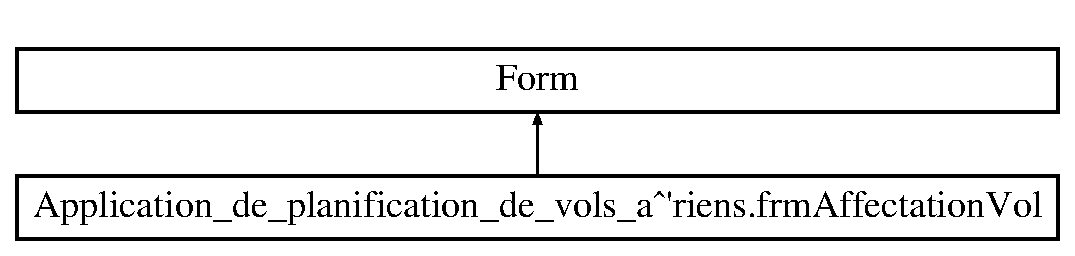
\includegraphics[height=2.000000cm]{class_application__de__planification__de__vols__a_xC3_xA9riens_1_1frm_affectation_vol}
\end{center}
\end{figure}
\subsection*{Public Member Functions}
\begin{DoxyCompactItemize}
\item 
\hyperlink{class_application__de__planification__de__vols__a_xC3_xA9riens_1_1frm_affectation_vol_aa24ceb68318baf83c2c5ed0661ac30dc}{frm\+Affectation\+Vol} ()
\end{DoxyCompactItemize}
\subsection*{Protected Member Functions}
\begin{DoxyCompactItemize}
\item 
override void \hyperlink{class_application__de__planification__de__vols__a_xC3_xA9riens_1_1frm_affectation_vol_a6964af23542006f8b01d264529a8298d}{Dispose} (bool disposing)
\begin{DoxyCompactList}\small\item\em Clean up any resources being used. \end{DoxyCompactList}\end{DoxyCompactItemize}


\subsection{Constructor \& Destructor Documentation}
\mbox{\Hypertarget{class_application__de__planification__de__vols__a_xC3_xA9riens_1_1frm_affectation_vol_aa24ceb68318baf83c2c5ed0661ac30dc}\label{class_application__de__planification__de__vols__a_xC3_xA9riens_1_1frm_affectation_vol_aa24ceb68318baf83c2c5ed0661ac30dc}} 
\index{Application\+\_\+de\+\_\+planification\+\_\+de\+\_\+vols\+\_\+aériens\+::frm\+Affectation\+Vol@{Application\+\_\+de\+\_\+planification\+\_\+de\+\_\+vols\+\_\+aériens\+::frm\+Affectation\+Vol}!frm\+Affectation\+Vol@{frm\+Affectation\+Vol}}
\index{frm\+Affectation\+Vol@{frm\+Affectation\+Vol}!Application\+\_\+de\+\_\+planification\+\_\+de\+\_\+vols\+\_\+aériens\+::frm\+Affectation\+Vol@{Application\+\_\+de\+\_\+planification\+\_\+de\+\_\+vols\+\_\+aériens\+::frm\+Affectation\+Vol}}
\subsubsection{\texorpdfstring{frm\+Affectation\+Vol()}{frmAffectationVol()}}
{\footnotesize\ttfamily Application\+\_\+de\+\_\+planification\+\_\+de\+\_\+vols\+\_\+aériens.\+frm\+Affectation\+Vol.\+frm\+Affectation\+Vol (\begin{DoxyParamCaption}{ }\end{DoxyParamCaption})}



\subsection{Member Function Documentation}
\mbox{\Hypertarget{class_application__de__planification__de__vols__a_xC3_xA9riens_1_1frm_affectation_vol_a6964af23542006f8b01d264529a8298d}\label{class_application__de__planification__de__vols__a_xC3_xA9riens_1_1frm_affectation_vol_a6964af23542006f8b01d264529a8298d}} 
\index{Application\+\_\+de\+\_\+planification\+\_\+de\+\_\+vols\+\_\+aériens\+::frm\+Affectation\+Vol@{Application\+\_\+de\+\_\+planification\+\_\+de\+\_\+vols\+\_\+aériens\+::frm\+Affectation\+Vol}!Dispose@{Dispose}}
\index{Dispose@{Dispose}!Application\+\_\+de\+\_\+planification\+\_\+de\+\_\+vols\+\_\+aériens\+::frm\+Affectation\+Vol@{Application\+\_\+de\+\_\+planification\+\_\+de\+\_\+vols\+\_\+aériens\+::frm\+Affectation\+Vol}}
\subsubsection{\texorpdfstring{Dispose()}{Dispose()}}
{\footnotesize\ttfamily override void Application\+\_\+de\+\_\+planification\+\_\+de\+\_\+vols\+\_\+aériens.\+frm\+Affectation\+Vol.\+Dispose (\begin{DoxyParamCaption}\item[{bool}]{disposing }\end{DoxyParamCaption})\hspace{0.3cm}{\ttfamily [protected]}}



Clean up any resources being used. 


\begin{DoxyParams}{Parameters}
{\em disposing} & true if managed resources should be disposed; otherwise, false.\\
\hline
\end{DoxyParams}


The documentation for this class was generated from the following files\+:\begin{DoxyCompactItemize}
\item 
Application de planification de vols aériens/\hyperlink{frm_affectation_vol_8cs}{frm\+Affectation\+Vol.\+cs}\item 
Application de planification de vols aériens/\hyperlink{frm_affectation_vol_8_designer_8cs}{frm\+Affectation\+Vol.\+Designer.\+cs}\end{DoxyCompactItemize}

\hypertarget{class_application__de__planification__de__vols__a_xC3_xA9riens_1_1frm_gestion}{}\section{Application\+\_\+de\+\_\+planification\+\_\+de\+\_\+vols\+\_\+aériens.\+frm\+Gestion Class Reference}
\label{class_application__de__planification__de__vols__a_xC3_xA9riens_1_1frm_gestion}\index{Application\+\_\+de\+\_\+planification\+\_\+de\+\_\+vols\+\_\+aériens.\+frm\+Gestion@{Application\+\_\+de\+\_\+planification\+\_\+de\+\_\+vols\+\_\+aériens.\+frm\+Gestion}}
Inheritance diagram for Application\+\_\+de\+\_\+planification\+\_\+de\+\_\+vols\+\_\+aériens.\+frm\+Gestion\+:\begin{figure}[H]
\begin{center}
\leavevmode
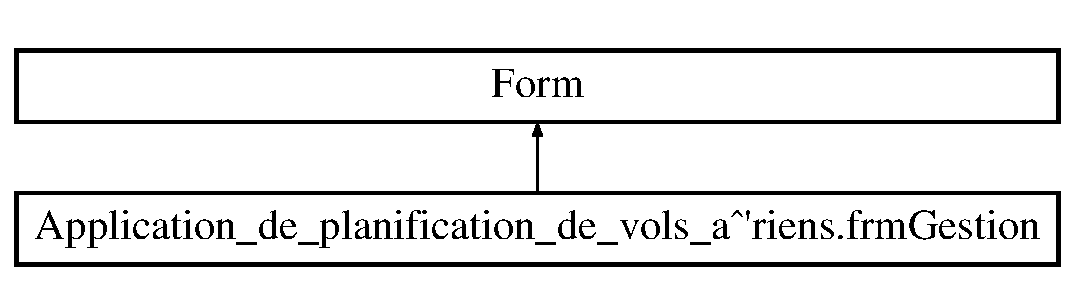
\includegraphics[height=2.000000cm]{class_application__de__planification__de__vols__a_xC3_xA9riens_1_1frm_gestion}
\end{center}
\end{figure}
\subsection*{Public Member Functions}
\begin{DoxyCompactItemize}
\item 
\hyperlink{class_application__de__planification__de__vols__a_xC3_xA9riens_1_1frm_gestion_aeb18ad09492b87eab030ed2f9179af97}{frm\+Gestion} ()
\end{DoxyCompactItemize}
\subsection*{Protected Member Functions}
\begin{DoxyCompactItemize}
\item 
override void \hyperlink{class_application__de__planification__de__vols__a_xC3_xA9riens_1_1frm_gestion_ae67280db69c5f87a5351f8729389d995}{Dispose} (bool disposing)
\begin{DoxyCompactList}\small\item\em Clean up any resources being used. \end{DoxyCompactList}\end{DoxyCompactItemize}


\subsection{Constructor \& Destructor Documentation}
\mbox{\Hypertarget{class_application__de__planification__de__vols__a_xC3_xA9riens_1_1frm_gestion_aeb18ad09492b87eab030ed2f9179af97}\label{class_application__de__planification__de__vols__a_xC3_xA9riens_1_1frm_gestion_aeb18ad09492b87eab030ed2f9179af97}} 
\index{Application\+\_\+de\+\_\+planification\+\_\+de\+\_\+vols\+\_\+aériens\+::frm\+Gestion@{Application\+\_\+de\+\_\+planification\+\_\+de\+\_\+vols\+\_\+aériens\+::frm\+Gestion}!frm\+Gestion@{frm\+Gestion}}
\index{frm\+Gestion@{frm\+Gestion}!Application\+\_\+de\+\_\+planification\+\_\+de\+\_\+vols\+\_\+aériens\+::frm\+Gestion@{Application\+\_\+de\+\_\+planification\+\_\+de\+\_\+vols\+\_\+aériens\+::frm\+Gestion}}
\subsubsection{\texorpdfstring{frm\+Gestion()}{frmGestion()}}
{\footnotesize\ttfamily Application\+\_\+de\+\_\+planification\+\_\+de\+\_\+vols\+\_\+aériens.\+frm\+Gestion.\+frm\+Gestion (\begin{DoxyParamCaption}{ }\end{DoxyParamCaption})}



\subsection{Member Function Documentation}
\mbox{\Hypertarget{class_application__de__planification__de__vols__a_xC3_xA9riens_1_1frm_gestion_ae67280db69c5f87a5351f8729389d995}\label{class_application__de__planification__de__vols__a_xC3_xA9riens_1_1frm_gestion_ae67280db69c5f87a5351f8729389d995}} 
\index{Application\+\_\+de\+\_\+planification\+\_\+de\+\_\+vols\+\_\+aériens\+::frm\+Gestion@{Application\+\_\+de\+\_\+planification\+\_\+de\+\_\+vols\+\_\+aériens\+::frm\+Gestion}!Dispose@{Dispose}}
\index{Dispose@{Dispose}!Application\+\_\+de\+\_\+planification\+\_\+de\+\_\+vols\+\_\+aériens\+::frm\+Gestion@{Application\+\_\+de\+\_\+planification\+\_\+de\+\_\+vols\+\_\+aériens\+::frm\+Gestion}}
\subsubsection{\texorpdfstring{Dispose()}{Dispose()}}
{\footnotesize\ttfamily override void Application\+\_\+de\+\_\+planification\+\_\+de\+\_\+vols\+\_\+aériens.\+frm\+Gestion.\+Dispose (\begin{DoxyParamCaption}\item[{bool}]{disposing }\end{DoxyParamCaption})\hspace{0.3cm}{\ttfamily [protected]}}



Clean up any resources being used. 


\begin{DoxyParams}{Parameters}
{\em disposing} & true if managed resources should be disposed; otherwise, false.\\
\hline
\end{DoxyParams}


The documentation for this class was generated from the following files\+:\begin{DoxyCompactItemize}
\item 
Application de planification de vols aériens/\hyperlink{frm_gestion_8cs}{frm\+Gestion.\+cs}\item 
Application de planification de vols aériens/\hyperlink{frm_gestion_8_designer_8cs}{frm\+Gestion.\+Designer.\+cs}\end{DoxyCompactItemize}

\hypertarget{class_application__de__planification__de__vols__a_xC3_xA9riens_1_1frm_vacances}{}\section{Application\+\_\+de\+\_\+planification\+\_\+de\+\_\+vols\+\_\+aériens.\+frm\+Vacances Class Reference}
\label{class_application__de__planification__de__vols__a_xC3_xA9riens_1_1frm_vacances}\index{Application\+\_\+de\+\_\+planification\+\_\+de\+\_\+vols\+\_\+aériens.\+frm\+Vacances@{Application\+\_\+de\+\_\+planification\+\_\+de\+\_\+vols\+\_\+aériens.\+frm\+Vacances}}
Inheritance diagram for Application\+\_\+de\+\_\+planification\+\_\+de\+\_\+vols\+\_\+aériens.\+frm\+Vacances\+:\begin{figure}[H]
\begin{center}
\leavevmode
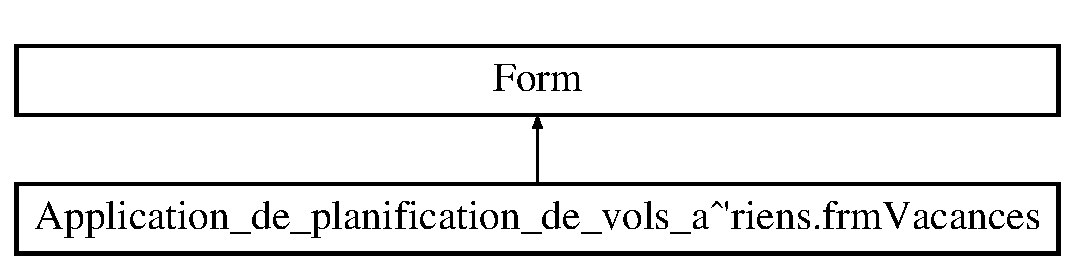
\includegraphics[height=2.000000cm]{class_application__de__planification__de__vols__a_xC3_xA9riens_1_1frm_vacances}
\end{center}
\end{figure}
\subsection*{Public Member Functions}
\begin{DoxyCompactItemize}
\item 
\hyperlink{class_application__de__planification__de__vols__a_xC3_xA9riens_1_1frm_vacances_af6ec175b735c98e670f562feb41dc256}{frm\+Vacances} ()
\end{DoxyCompactItemize}
\subsection*{Protected Member Functions}
\begin{DoxyCompactItemize}
\item 
override void \hyperlink{class_application__de__planification__de__vols__a_xC3_xA9riens_1_1frm_vacances_a618e271102d37f12ad7dad5d252e2492}{Dispose} (bool disposing)
\begin{DoxyCompactList}\small\item\em Clean up any resources being used. \end{DoxyCompactList}\end{DoxyCompactItemize}


\subsection{Constructor \& Destructor Documentation}
\mbox{\Hypertarget{class_application__de__planification__de__vols__a_xC3_xA9riens_1_1frm_vacances_af6ec175b735c98e670f562feb41dc256}\label{class_application__de__planification__de__vols__a_xC3_xA9riens_1_1frm_vacances_af6ec175b735c98e670f562feb41dc256}} 
\index{Application\+\_\+de\+\_\+planification\+\_\+de\+\_\+vols\+\_\+aériens\+::frm\+Vacances@{Application\+\_\+de\+\_\+planification\+\_\+de\+\_\+vols\+\_\+aériens\+::frm\+Vacances}!frm\+Vacances@{frm\+Vacances}}
\index{frm\+Vacances@{frm\+Vacances}!Application\+\_\+de\+\_\+planification\+\_\+de\+\_\+vols\+\_\+aériens\+::frm\+Vacances@{Application\+\_\+de\+\_\+planification\+\_\+de\+\_\+vols\+\_\+aériens\+::frm\+Vacances}}
\subsubsection{\texorpdfstring{frm\+Vacances()}{frmVacances()}}
{\footnotesize\ttfamily Application\+\_\+de\+\_\+planification\+\_\+de\+\_\+vols\+\_\+aériens.\+frm\+Vacances.\+frm\+Vacances (\begin{DoxyParamCaption}{ }\end{DoxyParamCaption})}



\subsection{Member Function Documentation}
\mbox{\Hypertarget{class_application__de__planification__de__vols__a_xC3_xA9riens_1_1frm_vacances_a618e271102d37f12ad7dad5d252e2492}\label{class_application__de__planification__de__vols__a_xC3_xA9riens_1_1frm_vacances_a618e271102d37f12ad7dad5d252e2492}} 
\index{Application\+\_\+de\+\_\+planification\+\_\+de\+\_\+vols\+\_\+aériens\+::frm\+Vacances@{Application\+\_\+de\+\_\+planification\+\_\+de\+\_\+vols\+\_\+aériens\+::frm\+Vacances}!Dispose@{Dispose}}
\index{Dispose@{Dispose}!Application\+\_\+de\+\_\+planification\+\_\+de\+\_\+vols\+\_\+aériens\+::frm\+Vacances@{Application\+\_\+de\+\_\+planification\+\_\+de\+\_\+vols\+\_\+aériens\+::frm\+Vacances}}
\subsubsection{\texorpdfstring{Dispose()}{Dispose()}}
{\footnotesize\ttfamily override void Application\+\_\+de\+\_\+planification\+\_\+de\+\_\+vols\+\_\+aériens.\+frm\+Vacances.\+Dispose (\begin{DoxyParamCaption}\item[{bool}]{disposing }\end{DoxyParamCaption})\hspace{0.3cm}{\ttfamily [protected]}}



Clean up any resources being used. 


\begin{DoxyParams}{Parameters}
{\em disposing} & true if managed resources should be disposed; otherwise, false.\\
\hline
\end{DoxyParams}


The documentation for this class was generated from the following files\+:\begin{DoxyCompactItemize}
\item 
Application de planification de vols aériens/\hyperlink{frm_vacances_8cs}{frm\+Vacances.\+cs}\item 
Application de planification de vols aériens/\hyperlink{frm_vacances_8_designer_8cs}{frm\+Vacances.\+Designer.\+cs}\end{DoxyCompactItemize}

\hypertarget{class_application__de__planification__de__vols__a_xC3_xA9riens_1_1frm_vacances_affichage}{}\section{Application\+\_\+de\+\_\+planification\+\_\+de\+\_\+vols\+\_\+aériens.\+frm\+Vacances\+Affichage Class Reference}
\label{class_application__de__planification__de__vols__a_xC3_xA9riens_1_1frm_vacances_affichage}\index{Application\+\_\+de\+\_\+planification\+\_\+de\+\_\+vols\+\_\+aériens.\+frm\+Vacances\+Affichage@{Application\+\_\+de\+\_\+planification\+\_\+de\+\_\+vols\+\_\+aériens.\+frm\+Vacances\+Affichage}}
Inheritance diagram for Application\+\_\+de\+\_\+planification\+\_\+de\+\_\+vols\+\_\+aériens.\+frm\+Vacances\+Affichage\+:\begin{figure}[H]
\begin{center}
\leavevmode
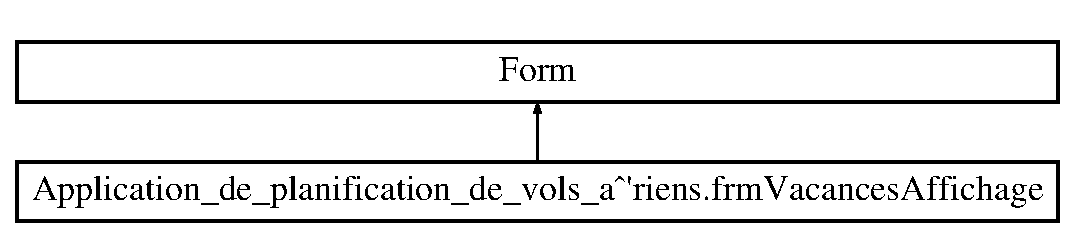
\includegraphics[height=2.000000cm]{class_application__de__planification__de__vols__a_xC3_xA9riens_1_1frm_vacances_affichage}
\end{center}
\end{figure}
\subsection*{Public Member Functions}
\begin{DoxyCompactItemize}
\item 
\hyperlink{class_application__de__planification__de__vols__a_xC3_xA9riens_1_1frm_vacances_affichage_a57aef6187251bbd4621c83517a46a73f}{frm\+Vacances\+Affichage} ()
\end{DoxyCompactItemize}
\subsection*{Protected Member Functions}
\begin{DoxyCompactItemize}
\item 
override void \hyperlink{class_application__de__planification__de__vols__a_xC3_xA9riens_1_1frm_vacances_affichage_afc0b73ee79ce33aadb85a91c77c9ce0e}{Dispose} (bool disposing)
\begin{DoxyCompactList}\small\item\em Clean up any resources being used. \end{DoxyCompactList}\end{DoxyCompactItemize}


\subsection{Constructor \& Destructor Documentation}
\mbox{\Hypertarget{class_application__de__planification__de__vols__a_xC3_xA9riens_1_1frm_vacances_affichage_a57aef6187251bbd4621c83517a46a73f}\label{class_application__de__planification__de__vols__a_xC3_xA9riens_1_1frm_vacances_affichage_a57aef6187251bbd4621c83517a46a73f}} 
\index{Application\+\_\+de\+\_\+planification\+\_\+de\+\_\+vols\+\_\+aériens\+::frm\+Vacances\+Affichage@{Application\+\_\+de\+\_\+planification\+\_\+de\+\_\+vols\+\_\+aériens\+::frm\+Vacances\+Affichage}!frm\+Vacances\+Affichage@{frm\+Vacances\+Affichage}}
\index{frm\+Vacances\+Affichage@{frm\+Vacances\+Affichage}!Application\+\_\+de\+\_\+planification\+\_\+de\+\_\+vols\+\_\+aériens\+::frm\+Vacances\+Affichage@{Application\+\_\+de\+\_\+planification\+\_\+de\+\_\+vols\+\_\+aériens\+::frm\+Vacances\+Affichage}}
\subsubsection{\texorpdfstring{frm\+Vacances\+Affichage()}{frmVacancesAffichage()}}
{\footnotesize\ttfamily Application\+\_\+de\+\_\+planification\+\_\+de\+\_\+vols\+\_\+aériens.\+frm\+Vacances\+Affichage.\+frm\+Vacances\+Affichage (\begin{DoxyParamCaption}{ }\end{DoxyParamCaption})}



\subsection{Member Function Documentation}
\mbox{\Hypertarget{class_application__de__planification__de__vols__a_xC3_xA9riens_1_1frm_vacances_affichage_afc0b73ee79ce33aadb85a91c77c9ce0e}\label{class_application__de__planification__de__vols__a_xC3_xA9riens_1_1frm_vacances_affichage_afc0b73ee79ce33aadb85a91c77c9ce0e}} 
\index{Application\+\_\+de\+\_\+planification\+\_\+de\+\_\+vols\+\_\+aériens\+::frm\+Vacances\+Affichage@{Application\+\_\+de\+\_\+planification\+\_\+de\+\_\+vols\+\_\+aériens\+::frm\+Vacances\+Affichage}!Dispose@{Dispose}}
\index{Dispose@{Dispose}!Application\+\_\+de\+\_\+planification\+\_\+de\+\_\+vols\+\_\+aériens\+::frm\+Vacances\+Affichage@{Application\+\_\+de\+\_\+planification\+\_\+de\+\_\+vols\+\_\+aériens\+::frm\+Vacances\+Affichage}}
\subsubsection{\texorpdfstring{Dispose()}{Dispose()}}
{\footnotesize\ttfamily override void Application\+\_\+de\+\_\+planification\+\_\+de\+\_\+vols\+\_\+aériens.\+frm\+Vacances\+Affichage.\+Dispose (\begin{DoxyParamCaption}\item[{bool}]{disposing }\end{DoxyParamCaption})\hspace{0.3cm}{\ttfamily [protected]}}



Clean up any resources being used. 


\begin{DoxyParams}{Parameters}
{\em disposing} & true if managed resources should be disposed; otherwise, false.\\
\hline
\end{DoxyParams}


The documentation for this class was generated from the following files\+:\begin{DoxyCompactItemize}
\item 
Application de planification de vols aériens/\hyperlink{frm_vacances_affichage_8cs}{frm\+Vacances\+Affichage.\+cs}\item 
Application de planification de vols aériens/\hyperlink{frm_vacances_affichage_8_designer_8cs}{frm\+Vacances\+Affichage.\+Designer.\+cs}\end{DoxyCompactItemize}

\hypertarget{class_application__de__planification__de__vols__a_xC3_xA9riens_1_1_line}{}\section{Application\+\_\+de\+\_\+planification\+\_\+de\+\_\+vols\+\_\+aériens.\+Line Class Reference}
\label{class_application__de__planification__de__vols__a_xC3_xA9riens_1_1_line}\index{Application\+\_\+de\+\_\+planification\+\_\+de\+\_\+vols\+\_\+aériens.\+Line@{Application\+\_\+de\+\_\+planification\+\_\+de\+\_\+vols\+\_\+aériens.\+Line}}
\subsection*{Public Member Functions}
\begin{DoxyCompactItemize}
\item 
\hyperlink{class_application__de__planification__de__vols__a_xC3_xA9riens_1_1_line_ac5938e9893f26cf7224e4bc65e919bb7}{Line} (\hyperlink{class_application__de__planification__de__vols__a_xC3_xA9riens_1_1_airport}{Airport} departure\+Airport, \hyperlink{class_application__de__planification__de__vols__a_xC3_xA9riens_1_1_airport}{Airport} arrival\+Airport, string distance)
\end{DoxyCompactItemize}
\subsection*{Properties}
\begin{DoxyCompactItemize}
\item 
string \hyperlink{class_application__de__planification__de__vols__a_xC3_xA9riens_1_1_line_ab20aa426dca4af775b0029f44c9b607d}{Distance}\hspace{0.3cm}{\ttfamily  \mbox{[}get, set\mbox{]}}
\end{DoxyCompactItemize}


\subsection{Constructor \& Destructor Documentation}
\mbox{\Hypertarget{class_application__de__planification__de__vols__a_xC3_xA9riens_1_1_line_ac5938e9893f26cf7224e4bc65e919bb7}\label{class_application__de__planification__de__vols__a_xC3_xA9riens_1_1_line_ac5938e9893f26cf7224e4bc65e919bb7}} 
\index{Application\+\_\+de\+\_\+planification\+\_\+de\+\_\+vols\+\_\+aériens\+::\+Line@{Application\+\_\+de\+\_\+planification\+\_\+de\+\_\+vols\+\_\+aériens\+::\+Line}!Line@{Line}}
\index{Line@{Line}!Application\+\_\+de\+\_\+planification\+\_\+de\+\_\+vols\+\_\+aériens\+::\+Line@{Application\+\_\+de\+\_\+planification\+\_\+de\+\_\+vols\+\_\+aériens\+::\+Line}}
\subsubsection{\texorpdfstring{Line()}{Line()}}
{\footnotesize\ttfamily Application\+\_\+de\+\_\+planification\+\_\+de\+\_\+vols\+\_\+aériens.\+Line.\+Line (\begin{DoxyParamCaption}\item[{\hyperlink{class_application__de__planification__de__vols__a_xC3_xA9riens_1_1_airport}{Airport}}]{departure\+Airport,  }\item[{\hyperlink{class_application__de__planification__de__vols__a_xC3_xA9riens_1_1_airport}{Airport}}]{arrival\+Airport,  }\item[{string}]{distance }\end{DoxyParamCaption})}



\subsection{Property Documentation}
\mbox{\Hypertarget{class_application__de__planification__de__vols__a_xC3_xA9riens_1_1_line_ab20aa426dca4af775b0029f44c9b607d}\label{class_application__de__planification__de__vols__a_xC3_xA9riens_1_1_line_ab20aa426dca4af775b0029f44c9b607d}} 
\index{Application\+\_\+de\+\_\+planification\+\_\+de\+\_\+vols\+\_\+aériens\+::\+Line@{Application\+\_\+de\+\_\+planification\+\_\+de\+\_\+vols\+\_\+aériens\+::\+Line}!Distance@{Distance}}
\index{Distance@{Distance}!Application\+\_\+de\+\_\+planification\+\_\+de\+\_\+vols\+\_\+aériens\+::\+Line@{Application\+\_\+de\+\_\+planification\+\_\+de\+\_\+vols\+\_\+aériens\+::\+Line}}
\subsubsection{\texorpdfstring{Distance}{Distance}}
{\footnotesize\ttfamily string Application\+\_\+de\+\_\+planification\+\_\+de\+\_\+vols\+\_\+aériens.\+Line.\+Distance\hspace{0.3cm}{\ttfamily [get]}, {\ttfamily [set]}}



The documentation for this class was generated from the following file\+:\begin{DoxyCompactItemize}
\item 
Application de planification de vols aériens/\hyperlink{_line_8cs}{Line.\+cs}\end{DoxyCompactItemize}

\hypertarget{class_application__de__planification__de__vols__a_xC3_xA9riens_1_1_pilot}{}\section{Application\+\_\+de\+\_\+planification\+\_\+de\+\_\+vols\+\_\+aériens.\+Pilot Class Reference}
\label{class_application__de__planification__de__vols__a_xC3_xA9riens_1_1_pilot}\index{Application\+\_\+de\+\_\+planification\+\_\+de\+\_\+vols\+\_\+aériens.\+Pilot@{Application\+\_\+de\+\_\+planification\+\_\+de\+\_\+vols\+\_\+aériens.\+Pilot}}
\subsection*{Public Member Functions}
\begin{DoxyCompactItemize}
\item 
\hyperlink{class_application__de__planification__de__vols__a_xC3_xA9riens_1_1_pilot_a7275b993fad3162863a8f8418c9e721b}{Pilot} (string name, string first\+Name, int flight\+Time, \hyperlink{class_application__de__planification__de__vols__a_xC3_xA9riens_1_1_airport}{Airport} assignment\+Airport)
\end{DoxyCompactItemize}
\subsection*{Properties}
\begin{DoxyCompactItemize}
\item 
string \hyperlink{class_application__de__planification__de__vols__a_xC3_xA9riens_1_1_pilot_a397bc161362554d9b1d76cf134255b14}{Name}\hspace{0.3cm}{\ttfamily  \mbox{[}get, set\mbox{]}}
\item 
string \hyperlink{class_application__de__planification__de__vols__a_xC3_xA9riens_1_1_pilot_ab3e8006344beff2d6f8c0c83e20aeaa1}{First\+Name}\hspace{0.3cm}{\ttfamily  \mbox{[}get, set\mbox{]}}
\item 
int \hyperlink{class_application__de__planification__de__vols__a_xC3_xA9riens_1_1_pilot_a04a6b4cd1e16d07382bef7536c5cf31e}{Flight\+Time}\hspace{0.3cm}{\ttfamily  \mbox{[}get, set\mbox{]}}
\item 
\hyperlink{class_application__de__planification__de__vols__a_xC3_xA9riens_1_1_airport}{Airport} \hyperlink{class_application__de__planification__de__vols__a_xC3_xA9riens_1_1_pilot_a451a7371cde9b8ddbae1a2119b0a4061}{Assignment\+Airport}\hspace{0.3cm}{\ttfamily  \mbox{[}get, set\mbox{]}}
\end{DoxyCompactItemize}


\subsection{Constructor \& Destructor Documentation}
\mbox{\Hypertarget{class_application__de__planification__de__vols__a_xC3_xA9riens_1_1_pilot_a7275b993fad3162863a8f8418c9e721b}\label{class_application__de__planification__de__vols__a_xC3_xA9riens_1_1_pilot_a7275b993fad3162863a8f8418c9e721b}} 
\index{Application\+\_\+de\+\_\+planification\+\_\+de\+\_\+vols\+\_\+aériens\+::\+Pilot@{Application\+\_\+de\+\_\+planification\+\_\+de\+\_\+vols\+\_\+aériens\+::\+Pilot}!Pilot@{Pilot}}
\index{Pilot@{Pilot}!Application\+\_\+de\+\_\+planification\+\_\+de\+\_\+vols\+\_\+aériens\+::\+Pilot@{Application\+\_\+de\+\_\+planification\+\_\+de\+\_\+vols\+\_\+aériens\+::\+Pilot}}
\subsubsection{\texorpdfstring{Pilot()}{Pilot()}}
{\footnotesize\ttfamily Application\+\_\+de\+\_\+planification\+\_\+de\+\_\+vols\+\_\+aériens.\+Pilot.\+Pilot (\begin{DoxyParamCaption}\item[{string}]{name,  }\item[{string}]{first\+Name,  }\item[{int}]{flight\+Time,  }\item[{\hyperlink{class_application__de__planification__de__vols__a_xC3_xA9riens_1_1_airport}{Airport}}]{assignment\+Airport }\end{DoxyParamCaption})}



\subsection{Property Documentation}
\mbox{\Hypertarget{class_application__de__planification__de__vols__a_xC3_xA9riens_1_1_pilot_a451a7371cde9b8ddbae1a2119b0a4061}\label{class_application__de__planification__de__vols__a_xC3_xA9riens_1_1_pilot_a451a7371cde9b8ddbae1a2119b0a4061}} 
\index{Application\+\_\+de\+\_\+planification\+\_\+de\+\_\+vols\+\_\+aériens\+::\+Pilot@{Application\+\_\+de\+\_\+planification\+\_\+de\+\_\+vols\+\_\+aériens\+::\+Pilot}!Assignment\+Airport@{Assignment\+Airport}}
\index{Assignment\+Airport@{Assignment\+Airport}!Application\+\_\+de\+\_\+planification\+\_\+de\+\_\+vols\+\_\+aériens\+::\+Pilot@{Application\+\_\+de\+\_\+planification\+\_\+de\+\_\+vols\+\_\+aériens\+::\+Pilot}}
\subsubsection{\texorpdfstring{Assignment\+Airport}{AssignmentAirport}}
{\footnotesize\ttfamily \hyperlink{class_application__de__planification__de__vols__a_xC3_xA9riens_1_1_airport}{Airport} Application\+\_\+de\+\_\+planification\+\_\+de\+\_\+vols\+\_\+aériens.\+Pilot.\+Assignment\+Airport\hspace{0.3cm}{\ttfamily [get]}, {\ttfamily [set]}}

\mbox{\Hypertarget{class_application__de__planification__de__vols__a_xC3_xA9riens_1_1_pilot_ab3e8006344beff2d6f8c0c83e20aeaa1}\label{class_application__de__planification__de__vols__a_xC3_xA9riens_1_1_pilot_ab3e8006344beff2d6f8c0c83e20aeaa1}} 
\index{Application\+\_\+de\+\_\+planification\+\_\+de\+\_\+vols\+\_\+aériens\+::\+Pilot@{Application\+\_\+de\+\_\+planification\+\_\+de\+\_\+vols\+\_\+aériens\+::\+Pilot}!First\+Name@{First\+Name}}
\index{First\+Name@{First\+Name}!Application\+\_\+de\+\_\+planification\+\_\+de\+\_\+vols\+\_\+aériens\+::\+Pilot@{Application\+\_\+de\+\_\+planification\+\_\+de\+\_\+vols\+\_\+aériens\+::\+Pilot}}
\subsubsection{\texorpdfstring{First\+Name}{FirstName}}
{\footnotesize\ttfamily string Application\+\_\+de\+\_\+planification\+\_\+de\+\_\+vols\+\_\+aériens.\+Pilot.\+First\+Name\hspace{0.3cm}{\ttfamily [get]}, {\ttfamily [set]}}

\mbox{\Hypertarget{class_application__de__planification__de__vols__a_xC3_xA9riens_1_1_pilot_a04a6b4cd1e16d07382bef7536c5cf31e}\label{class_application__de__planification__de__vols__a_xC3_xA9riens_1_1_pilot_a04a6b4cd1e16d07382bef7536c5cf31e}} 
\index{Application\+\_\+de\+\_\+planification\+\_\+de\+\_\+vols\+\_\+aériens\+::\+Pilot@{Application\+\_\+de\+\_\+planification\+\_\+de\+\_\+vols\+\_\+aériens\+::\+Pilot}!Flight\+Time@{Flight\+Time}}
\index{Flight\+Time@{Flight\+Time}!Application\+\_\+de\+\_\+planification\+\_\+de\+\_\+vols\+\_\+aériens\+::\+Pilot@{Application\+\_\+de\+\_\+planification\+\_\+de\+\_\+vols\+\_\+aériens\+::\+Pilot}}
\subsubsection{\texorpdfstring{Flight\+Time}{FlightTime}}
{\footnotesize\ttfamily int Application\+\_\+de\+\_\+planification\+\_\+de\+\_\+vols\+\_\+aériens.\+Pilot.\+Flight\+Time\hspace{0.3cm}{\ttfamily [get]}, {\ttfamily [set]}}

\mbox{\Hypertarget{class_application__de__planification__de__vols__a_xC3_xA9riens_1_1_pilot_a397bc161362554d9b1d76cf134255b14}\label{class_application__de__planification__de__vols__a_xC3_xA9riens_1_1_pilot_a397bc161362554d9b1d76cf134255b14}} 
\index{Application\+\_\+de\+\_\+planification\+\_\+de\+\_\+vols\+\_\+aériens\+::\+Pilot@{Application\+\_\+de\+\_\+planification\+\_\+de\+\_\+vols\+\_\+aériens\+::\+Pilot}!Name@{Name}}
\index{Name@{Name}!Application\+\_\+de\+\_\+planification\+\_\+de\+\_\+vols\+\_\+aériens\+::\+Pilot@{Application\+\_\+de\+\_\+planification\+\_\+de\+\_\+vols\+\_\+aériens\+::\+Pilot}}
\subsubsection{\texorpdfstring{Name}{Name}}
{\footnotesize\ttfamily string Application\+\_\+de\+\_\+planification\+\_\+de\+\_\+vols\+\_\+aériens.\+Pilot.\+Name\hspace{0.3cm}{\ttfamily [get]}, {\ttfamily [set]}}



The documentation for this class was generated from the following file\+:\begin{DoxyCompactItemize}
\item 
Application de planification de vols aériens/\hyperlink{_pilot_8cs}{Pilot.\+cs}\end{DoxyCompactItemize}

\hypertarget{class_application__de__planification__de__vols__a_xC3_xA9riens_1_1_program}{}\section{Application\+\_\+de\+\_\+planification\+\_\+de\+\_\+vols\+\_\+aériens.\+Program Class Reference}
\label{class_application__de__planification__de__vols__a_xC3_xA9riens_1_1_program}\index{Application\+\_\+de\+\_\+planification\+\_\+de\+\_\+vols\+\_\+aériens.\+Program@{Application\+\_\+de\+\_\+planification\+\_\+de\+\_\+vols\+\_\+aériens.\+Program}}


The documentation for this class was generated from the following file\+:\begin{DoxyCompactItemize}
\item 
Application de planification de vols aériens/\hyperlink{_program_8cs}{Program.\+cs}\end{DoxyCompactItemize}

\hypertarget{class_application__de__planification__de__vols__a_xC3_xA9riens_1_1_vacation}{}\section{Application\+\_\+de\+\_\+planification\+\_\+de\+\_\+vols\+\_\+aériens.\+Vacation Class Reference}
\label{class_application__de__planification__de__vols__a_xC3_xA9riens_1_1_vacation}\index{Application\+\_\+de\+\_\+planification\+\_\+de\+\_\+vols\+\_\+aériens.\+Vacation@{Application\+\_\+de\+\_\+planification\+\_\+de\+\_\+vols\+\_\+aériens.\+Vacation}}
\subsection*{Public Member Functions}
\begin{DoxyCompactItemize}
\item 
\hyperlink{class_application__de__planification__de__vols__a_xC3_xA9riens_1_1_vacation_abd1900c4e75c89a0a681c8fd83d6f6fc}{Vacation} (Date\+Time start\+Date, Date\+Time end\+Date, \hyperlink{class_application__de__planification__de__vols__a_xC3_xA9riens_1_1_pilot}{Pilot} pilot)
\end{DoxyCompactItemize}
\subsection*{Properties}
\begin{DoxyCompactItemize}
\item 
Date\+Time \hyperlink{class_application__de__planification__de__vols__a_xC3_xA9riens_1_1_vacation_a5ebeb112b3fffb8c5325ac0ce7000ad6}{Start\+Date}\hspace{0.3cm}{\ttfamily  \mbox{[}get, set\mbox{]}}
\item 
Date\+Time \hyperlink{class_application__de__planification__de__vols__a_xC3_xA9riens_1_1_vacation_ae255a27724aa8d84aee0fa8ec23a4878}{End\+Date}\hspace{0.3cm}{\ttfamily  \mbox{[}get, set\mbox{]}}
\item 
\hyperlink{class_application__de__planification__de__vols__a_xC3_xA9riens_1_1_pilot}{Pilot} \hyperlink{class_application__de__planification__de__vols__a_xC3_xA9riens_1_1_vacation_a87be5d673051905ea03c547cb55ec866}{Pilot}\hspace{0.3cm}{\ttfamily  \mbox{[}get, set\mbox{]}}
\end{DoxyCompactItemize}


\subsection{Constructor \& Destructor Documentation}
\mbox{\Hypertarget{class_application__de__planification__de__vols__a_xC3_xA9riens_1_1_vacation_abd1900c4e75c89a0a681c8fd83d6f6fc}\label{class_application__de__planification__de__vols__a_xC3_xA9riens_1_1_vacation_abd1900c4e75c89a0a681c8fd83d6f6fc}} 
\index{Application\+\_\+de\+\_\+planification\+\_\+de\+\_\+vols\+\_\+aériens\+::\+Vacation@{Application\+\_\+de\+\_\+planification\+\_\+de\+\_\+vols\+\_\+aériens\+::\+Vacation}!Vacation@{Vacation}}
\index{Vacation@{Vacation}!Application\+\_\+de\+\_\+planification\+\_\+de\+\_\+vols\+\_\+aériens\+::\+Vacation@{Application\+\_\+de\+\_\+planification\+\_\+de\+\_\+vols\+\_\+aériens\+::\+Vacation}}
\subsubsection{\texorpdfstring{Vacation()}{Vacation()}}
{\footnotesize\ttfamily Application\+\_\+de\+\_\+planification\+\_\+de\+\_\+vols\+\_\+aériens.\+Vacation.\+Vacation (\begin{DoxyParamCaption}\item[{Date\+Time}]{start\+Date,  }\item[{Date\+Time}]{end\+Date,  }\item[{\hyperlink{class_application__de__planification__de__vols__a_xC3_xA9riens_1_1_pilot}{Pilot}}]{pilot }\end{DoxyParamCaption})}



\subsection{Property Documentation}
\mbox{\Hypertarget{class_application__de__planification__de__vols__a_xC3_xA9riens_1_1_vacation_ae255a27724aa8d84aee0fa8ec23a4878}\label{class_application__de__planification__de__vols__a_xC3_xA9riens_1_1_vacation_ae255a27724aa8d84aee0fa8ec23a4878}} 
\index{Application\+\_\+de\+\_\+planification\+\_\+de\+\_\+vols\+\_\+aériens\+::\+Vacation@{Application\+\_\+de\+\_\+planification\+\_\+de\+\_\+vols\+\_\+aériens\+::\+Vacation}!End\+Date@{End\+Date}}
\index{End\+Date@{End\+Date}!Application\+\_\+de\+\_\+planification\+\_\+de\+\_\+vols\+\_\+aériens\+::\+Vacation@{Application\+\_\+de\+\_\+planification\+\_\+de\+\_\+vols\+\_\+aériens\+::\+Vacation}}
\subsubsection{\texorpdfstring{End\+Date}{EndDate}}
{\footnotesize\ttfamily Date\+Time Application\+\_\+de\+\_\+planification\+\_\+de\+\_\+vols\+\_\+aériens.\+Vacation.\+End\+Date\hspace{0.3cm}{\ttfamily [get]}, {\ttfamily [set]}}

\mbox{\Hypertarget{class_application__de__planification__de__vols__a_xC3_xA9riens_1_1_vacation_a87be5d673051905ea03c547cb55ec866}\label{class_application__de__planification__de__vols__a_xC3_xA9riens_1_1_vacation_a87be5d673051905ea03c547cb55ec866}} 
\index{Application\+\_\+de\+\_\+planification\+\_\+de\+\_\+vols\+\_\+aériens\+::\+Vacation@{Application\+\_\+de\+\_\+planification\+\_\+de\+\_\+vols\+\_\+aériens\+::\+Vacation}!Pilot@{Pilot}}
\index{Pilot@{Pilot}!Application\+\_\+de\+\_\+planification\+\_\+de\+\_\+vols\+\_\+aériens\+::\+Vacation@{Application\+\_\+de\+\_\+planification\+\_\+de\+\_\+vols\+\_\+aériens\+::\+Vacation}}
\subsubsection{\texorpdfstring{Pilot}{Pilot}}
{\footnotesize\ttfamily \hyperlink{class_application__de__planification__de__vols__a_xC3_xA9riens_1_1_pilot}{Pilot} Application\+\_\+de\+\_\+planification\+\_\+de\+\_\+vols\+\_\+aériens.\+Vacation.\+Pilot\hspace{0.3cm}{\ttfamily [get]}, {\ttfamily [set]}}

\mbox{\Hypertarget{class_application__de__planification__de__vols__a_xC3_xA9riens_1_1_vacation_a5ebeb112b3fffb8c5325ac0ce7000ad6}\label{class_application__de__planification__de__vols__a_xC3_xA9riens_1_1_vacation_a5ebeb112b3fffb8c5325ac0ce7000ad6}} 
\index{Application\+\_\+de\+\_\+planification\+\_\+de\+\_\+vols\+\_\+aériens\+::\+Vacation@{Application\+\_\+de\+\_\+planification\+\_\+de\+\_\+vols\+\_\+aériens\+::\+Vacation}!Start\+Date@{Start\+Date}}
\index{Start\+Date@{Start\+Date}!Application\+\_\+de\+\_\+planification\+\_\+de\+\_\+vols\+\_\+aériens\+::\+Vacation@{Application\+\_\+de\+\_\+planification\+\_\+de\+\_\+vols\+\_\+aériens\+::\+Vacation}}
\subsubsection{\texorpdfstring{Start\+Date}{StartDate}}
{\footnotesize\ttfamily Date\+Time Application\+\_\+de\+\_\+planification\+\_\+de\+\_\+vols\+\_\+aériens.\+Vacation.\+Start\+Date\hspace{0.3cm}{\ttfamily [get]}, {\ttfamily [set]}}



The documentation for this class was generated from the following file\+:\begin{DoxyCompactItemize}
\item 
Application de planification de vols aériens/\hyperlink{_vacation_8cs}{Vacation.\+cs}\end{DoxyCompactItemize}

\chapter{File Documentation}
\hypertarget{_airport_8cs}{}\section{Application de planification de vols aériens/\+Airport.cs File Reference}
\label{_airport_8cs}\index{Application de planification de vols aériens/\+Airport.\+cs@{Application de planification de vols aériens/\+Airport.\+cs}}
\subsection*{Classes}
\begin{DoxyCompactItemize}
\item 
class \hyperlink{class_application__de__planification__de__vols__a_xC3_xA9riens_1_1_airport}{Application\+\_\+de\+\_\+planification\+\_\+de\+\_\+vols\+\_\+aériens.\+Airport}
\end{DoxyCompactItemize}
\subsection*{Namespaces}
\begin{DoxyCompactItemize}
\item 
namespace \hyperlink{namespace_application__de__planification__de__vols__a_xC3_xA9riens}{Application\+\_\+de\+\_\+planification\+\_\+de\+\_\+vols\+\_\+aériens}
\end{DoxyCompactItemize}

\hypertarget{_d_b_connexion_8cs}{}\section{Application de planification de vols aériens/\+D\+B\+Connexion.cs File Reference}
\label{_d_b_connexion_8cs}\index{Application de planification de vols aériens/\+D\+B\+Connexion.\+cs@{Application de planification de vols aériens/\+D\+B\+Connexion.\+cs}}
\subsection*{Classes}
\begin{DoxyCompactItemize}
\item 
class \hyperlink{class_application__de__planification__de__vols__a_xC3_xA9riens_1_1_d_b_connexion}{Application\+\_\+de\+\_\+planification\+\_\+de\+\_\+vols\+\_\+aériens.\+D\+B\+Connexion}
\end{DoxyCompactItemize}
\subsection*{Namespaces}
\begin{DoxyCompactItemize}
\item 
namespace \hyperlink{namespace_application__de__planification__de__vols__a_xC3_xA9riens}{Application\+\_\+de\+\_\+planification\+\_\+de\+\_\+vols\+\_\+aériens}
\end{DoxyCompactItemize}

\hypertarget{_flight_8cs}{}\section{Application de planification de vols aériens/\+Flight.cs File Reference}
\label{_flight_8cs}\index{Application de planification de vols aériens/\+Flight.\+cs@{Application de planification de vols aériens/\+Flight.\+cs}}
\subsection*{Classes}
\begin{DoxyCompactItemize}
\item 
class \hyperlink{class_application__de__planification__de__vols__a_xC3_xA9riens_1_1_flight}{Application\+\_\+de\+\_\+planification\+\_\+de\+\_\+vols\+\_\+aériens.\+Flight}
\end{DoxyCompactItemize}
\subsection*{Namespaces}
\begin{DoxyCompactItemize}
\item 
namespace \hyperlink{namespace_application__de__planification__de__vols__a_xC3_xA9riens}{Application\+\_\+de\+\_\+planification\+\_\+de\+\_\+vols\+\_\+aériens}
\end{DoxyCompactItemize}

\hypertarget{_flight_schedule_8cs}{}\section{Application de planification de vols aériens/\+Flight\+Schedule.cs File Reference}
\label{_flight_schedule_8cs}\index{Application de planification de vols aériens/\+Flight\+Schedule.\+cs@{Application de planification de vols aériens/\+Flight\+Schedule.\+cs}}
\subsection*{Classes}
\begin{DoxyCompactItemize}
\item 
class \hyperlink{class_application__de__planification__de__vols__a_xC3_xA9riens_1_1_flight_schedule}{Application\+\_\+de\+\_\+planification\+\_\+de\+\_\+vols\+\_\+aériens.\+Flight\+Schedule}
\end{DoxyCompactItemize}
\subsection*{Namespaces}
\begin{DoxyCompactItemize}
\item 
namespace \hyperlink{namespace_application__de__planification__de__vols__a_xC3_xA9riens}{Application\+\_\+de\+\_\+planification\+\_\+de\+\_\+vols\+\_\+aériens}
\end{DoxyCompactItemize}

\hypertarget{frm_affectation_vol_8cs}{}\section{Application de planification de vols aériens/frm\+Affectation\+Vol.cs File Reference}
\label{frm_affectation_vol_8cs}\index{Application de planification de vols aériens/frm\+Affectation\+Vol.\+cs@{Application de planification de vols aériens/frm\+Affectation\+Vol.\+cs}}
\subsection*{Classes}
\begin{DoxyCompactItemize}
\item 
class \hyperlink{class_application__de__planification__de__vols__a_xC3_xA9riens_1_1frm_affectation_vol}{Application\+\_\+de\+\_\+planification\+\_\+de\+\_\+vols\+\_\+aériens.\+frm\+Affectation\+Vol}
\end{DoxyCompactItemize}
\subsection*{Namespaces}
\begin{DoxyCompactItemize}
\item 
namespace \hyperlink{namespace_application__de__planification__de__vols__a_xC3_xA9riens}{Application\+\_\+de\+\_\+planification\+\_\+de\+\_\+vols\+\_\+aériens}
\end{DoxyCompactItemize}

\hypertarget{frm_affectation_vol_8_designer_8cs}{}\section{Application de planification de vols aériens/frm\+Affectation\+Vol.Designer.\+cs File Reference}
\label{frm_affectation_vol_8_designer_8cs}\index{Application de planification de vols aériens/frm\+Affectation\+Vol.\+Designer.\+cs@{Application de planification de vols aériens/frm\+Affectation\+Vol.\+Designer.\+cs}}
\subsection*{Classes}
\begin{DoxyCompactItemize}
\item 
class \hyperlink{class_application__de__planification__de__vols__a_xC3_xA9riens_1_1frm_affectation_vol}{Application\+\_\+de\+\_\+planification\+\_\+de\+\_\+vols\+\_\+aériens.\+frm\+Affectation\+Vol}
\end{DoxyCompactItemize}
\subsection*{Namespaces}
\begin{DoxyCompactItemize}
\item 
namespace \hyperlink{namespace_application__de__planification__de__vols__a_xC3_xA9riens}{Application\+\_\+de\+\_\+planification\+\_\+de\+\_\+vols\+\_\+aériens}
\end{DoxyCompactItemize}

\hypertarget{frm_affichage_8cs}{}\section{Application de planification de vols aériens/frm\+Affichage.cs File Reference}
\label{frm_affichage_8cs}\index{Application de planification de vols aériens/frm\+Affichage.\+cs@{Application de planification de vols aériens/frm\+Affichage.\+cs}}
\subsection*{Classes}
\begin{DoxyCompactItemize}
\item 
class \hyperlink{class_application__de__planification__de__vols__a_xC3_xA9riens_1_1_affichage}{Application\+\_\+de\+\_\+planification\+\_\+de\+\_\+vols\+\_\+aériens.\+Affichage}
\end{DoxyCompactItemize}
\subsection*{Namespaces}
\begin{DoxyCompactItemize}
\item 
namespace \hyperlink{namespace_application__de__planification__de__vols__a_xC3_xA9riens}{Application\+\_\+de\+\_\+planification\+\_\+de\+\_\+vols\+\_\+aériens}
\end{DoxyCompactItemize}

\hypertarget{frm_affichage_8_designer_8cs}{}\section{Application de planification de vols aériens/frm\+Affichage.Designer.\+cs File Reference}
\label{frm_affichage_8_designer_8cs}\index{Application de planification de vols aériens/frm\+Affichage.\+Designer.\+cs@{Application de planification de vols aériens/frm\+Affichage.\+Designer.\+cs}}
\subsection*{Classes}
\begin{DoxyCompactItemize}
\item 
class \hyperlink{class_application__de__planification__de__vols__a_xC3_xA9riens_1_1_affichage}{Application\+\_\+de\+\_\+planification\+\_\+de\+\_\+vols\+\_\+aériens.\+Affichage}
\end{DoxyCompactItemize}
\subsection*{Namespaces}
\begin{DoxyCompactItemize}
\item 
namespace \hyperlink{namespace_application__de__planification__de__vols__a_xC3_xA9riens}{Application\+\_\+de\+\_\+planification\+\_\+de\+\_\+vols\+\_\+aériens}
\end{DoxyCompactItemize}

\hypertarget{frm_gestion_8cs}{}\section{Application de planification de vols aériens/frm\+Gestion.cs File Reference}
\label{frm_gestion_8cs}\index{Application de planification de vols aériens/frm\+Gestion.\+cs@{Application de planification de vols aériens/frm\+Gestion.\+cs}}
\subsection*{Classes}
\begin{DoxyCompactItemize}
\item 
class \hyperlink{class_application__de__planification__de__vols__a_xC3_xA9riens_1_1frm_gestion}{Application\+\_\+de\+\_\+planification\+\_\+de\+\_\+vols\+\_\+aériens.\+frm\+Gestion}
\end{DoxyCompactItemize}
\subsection*{Namespaces}
\begin{DoxyCompactItemize}
\item 
namespace \hyperlink{namespace_application__de__planification__de__vols__a_xC3_xA9riens}{Application\+\_\+de\+\_\+planification\+\_\+de\+\_\+vols\+\_\+aériens}
\end{DoxyCompactItemize}

\hypertarget{frm_gestion_8_designer_8cs}{}\section{Application de planification de vols aériens/frm\+Gestion.Designer.\+cs File Reference}
\label{frm_gestion_8_designer_8cs}\index{Application de planification de vols aériens/frm\+Gestion.\+Designer.\+cs@{Application de planification de vols aériens/frm\+Gestion.\+Designer.\+cs}}
\subsection*{Classes}
\begin{DoxyCompactItemize}
\item 
class \hyperlink{class_application__de__planification__de__vols__a_xC3_xA9riens_1_1frm_gestion}{Application\+\_\+de\+\_\+planification\+\_\+de\+\_\+vols\+\_\+aériens.\+frm\+Gestion}
\end{DoxyCompactItemize}
\subsection*{Namespaces}
\begin{DoxyCompactItemize}
\item 
namespace \hyperlink{namespace_application__de__planification__de__vols__a_xC3_xA9riens}{Application\+\_\+de\+\_\+planification\+\_\+de\+\_\+vols\+\_\+aériens}
\end{DoxyCompactItemize}

\hypertarget{frm_vacances_8cs}{}\section{Application de planification de vols aériens/frm\+Vacances.cs File Reference}
\label{frm_vacances_8cs}\index{Application de planification de vols aériens/frm\+Vacances.\+cs@{Application de planification de vols aériens/frm\+Vacances.\+cs}}
\subsection*{Classes}
\begin{DoxyCompactItemize}
\item 
class \hyperlink{class_application__de__planification__de__vols__a_xC3_xA9riens_1_1frm_vacances}{Application\+\_\+de\+\_\+planification\+\_\+de\+\_\+vols\+\_\+aériens.\+frm\+Vacances}
\end{DoxyCompactItemize}
\subsection*{Namespaces}
\begin{DoxyCompactItemize}
\item 
namespace \hyperlink{namespace_application__de__planification__de__vols__a_xC3_xA9riens}{Application\+\_\+de\+\_\+planification\+\_\+de\+\_\+vols\+\_\+aériens}
\end{DoxyCompactItemize}

\hypertarget{frm_vacances_8_designer_8cs}{}\section{Application de planification de vols aériens/frm\+Vacances.Designer.\+cs File Reference}
\label{frm_vacances_8_designer_8cs}\index{Application de planification de vols aériens/frm\+Vacances.\+Designer.\+cs@{Application de planification de vols aériens/frm\+Vacances.\+Designer.\+cs}}
\subsection*{Classes}
\begin{DoxyCompactItemize}
\item 
class \hyperlink{class_application__de__planification__de__vols__a_xC3_xA9riens_1_1frm_vacances}{Application\+\_\+de\+\_\+planification\+\_\+de\+\_\+vols\+\_\+aériens.\+frm\+Vacances}
\end{DoxyCompactItemize}
\subsection*{Namespaces}
\begin{DoxyCompactItemize}
\item 
namespace \hyperlink{namespace_application__de__planification__de__vols__a_xC3_xA9riens}{Application\+\_\+de\+\_\+planification\+\_\+de\+\_\+vols\+\_\+aériens}
\end{DoxyCompactItemize}

\hypertarget{frm_vacances_affichage_8cs}{}\section{Application de planification de vols aériens/frm\+Vacances\+Affichage.cs File Reference}
\label{frm_vacances_affichage_8cs}\index{Application de planification de vols aériens/frm\+Vacances\+Affichage.\+cs@{Application de planification de vols aériens/frm\+Vacances\+Affichage.\+cs}}
\subsection*{Classes}
\begin{DoxyCompactItemize}
\item 
class \hyperlink{class_application__de__planification__de__vols__a_xC3_xA9riens_1_1frm_vacances_affichage}{Application\+\_\+de\+\_\+planification\+\_\+de\+\_\+vols\+\_\+aériens.\+frm\+Vacances\+Affichage}
\end{DoxyCompactItemize}
\subsection*{Namespaces}
\begin{DoxyCompactItemize}
\item 
namespace \hyperlink{namespace_application__de__planification__de__vols__a_xC3_xA9riens}{Application\+\_\+de\+\_\+planification\+\_\+de\+\_\+vols\+\_\+aériens}
\end{DoxyCompactItemize}

\hypertarget{frm_vacances_affichage_8_designer_8cs}{}\section{Application de planification de vols aériens/frm\+Vacances\+Affichage.Designer.\+cs File Reference}
\label{frm_vacances_affichage_8_designer_8cs}\index{Application de planification de vols aériens/frm\+Vacances\+Affichage.\+Designer.\+cs@{Application de planification de vols aériens/frm\+Vacances\+Affichage.\+Designer.\+cs}}
\subsection*{Classes}
\begin{DoxyCompactItemize}
\item 
class \hyperlink{class_application__de__planification__de__vols__a_xC3_xA9riens_1_1frm_vacances_affichage}{Application\+\_\+de\+\_\+planification\+\_\+de\+\_\+vols\+\_\+aériens.\+frm\+Vacances\+Affichage}
\end{DoxyCompactItemize}
\subsection*{Namespaces}
\begin{DoxyCompactItemize}
\item 
namespace \hyperlink{namespace_application__de__planification__de__vols__a_xC3_xA9riens}{Application\+\_\+de\+\_\+planification\+\_\+de\+\_\+vols\+\_\+aériens}
\end{DoxyCompactItemize}

\hypertarget{_line_8cs}{}\section{Application de planification de vols aériens/\+Line.cs File Reference}
\label{_line_8cs}\index{Application de planification de vols aériens/\+Line.\+cs@{Application de planification de vols aériens/\+Line.\+cs}}
\subsection*{Classes}
\begin{DoxyCompactItemize}
\item 
class \hyperlink{class_application__de__planification__de__vols__a_xC3_xA9riens_1_1_line}{Application\+\_\+de\+\_\+planification\+\_\+de\+\_\+vols\+\_\+aériens.\+Line}
\end{DoxyCompactItemize}
\subsection*{Namespaces}
\begin{DoxyCompactItemize}
\item 
namespace \hyperlink{namespace_application__de__planification__de__vols__a_xC3_xA9riens}{Application\+\_\+de\+\_\+planification\+\_\+de\+\_\+vols\+\_\+aériens}
\end{DoxyCompactItemize}

\hypertarget{_pilot_8cs}{}\section{Application de planification de vols aériens/\+Pilot.cs File Reference}
\label{_pilot_8cs}\index{Application de planification de vols aériens/\+Pilot.\+cs@{Application de planification de vols aériens/\+Pilot.\+cs}}
\subsection*{Classes}
\begin{DoxyCompactItemize}
\item 
class \hyperlink{class_application__de__planification__de__vols__a_xC3_xA9riens_1_1_pilot}{Application\+\_\+de\+\_\+planification\+\_\+de\+\_\+vols\+\_\+aériens.\+Pilot}
\end{DoxyCompactItemize}
\subsection*{Namespaces}
\begin{DoxyCompactItemize}
\item 
namespace \hyperlink{namespace_application__de__planification__de__vols__a_xC3_xA9riens}{Application\+\_\+de\+\_\+planification\+\_\+de\+\_\+vols\+\_\+aériens}
\end{DoxyCompactItemize}

\hypertarget{_program_8cs}{}\section{Application de planification de vols aériens/\+Program.cs File Reference}
\label{_program_8cs}\index{Application de planification de vols aériens/\+Program.\+cs@{Application de planification de vols aériens/\+Program.\+cs}}
\subsection*{Classes}
\begin{DoxyCompactItemize}
\item 
class \hyperlink{class_application__de__planification__de__vols__a_xC3_xA9riens_1_1_program}{Application\+\_\+de\+\_\+planification\+\_\+de\+\_\+vols\+\_\+aériens.\+Program}
\end{DoxyCompactItemize}
\subsection*{Namespaces}
\begin{DoxyCompactItemize}
\item 
namespace \hyperlink{namespace_application__de__planification__de__vols__a_xC3_xA9riens}{Application\+\_\+de\+\_\+planification\+\_\+de\+\_\+vols\+\_\+aériens}
\end{DoxyCompactItemize}

\hypertarget{_vacation_8cs}{}\section{Application de planification de vols aériens/\+Vacation.cs File Reference}
\label{_vacation_8cs}\index{Application de planification de vols aériens/\+Vacation.\+cs@{Application de planification de vols aériens/\+Vacation.\+cs}}
\subsection*{Classes}
\begin{DoxyCompactItemize}
\item 
class \hyperlink{class_application__de__planification__de__vols__a_xC3_xA9riens_1_1_vacation}{Application\+\_\+de\+\_\+planification\+\_\+de\+\_\+vols\+\_\+aériens.\+Vacation}
\end{DoxyCompactItemize}
\subsection*{Namespaces}
\begin{DoxyCompactItemize}
\item 
namespace \hyperlink{namespace_application__de__planification__de__vols__a_xC3_xA9riens}{Application\+\_\+de\+\_\+planification\+\_\+de\+\_\+vols\+\_\+aériens}
\end{DoxyCompactItemize}

%--- End generated contents ---

% Index
\backmatter
\newpage
\phantomsection
\clearemptydoublepage
\addcontentsline{toc}{chapter}{Index}
\printindex

\end{document}
